%************************************************
\chapter{Reflectively Learning to Control}
\label{chapter:reflectively_learning_to_control}
%************************************************

In order to explain my implemented solution to the problem of
reflectively learning-to-control, I will focus on a running example
within the physical block building domain shown in
\autoref{figure:an_example_problem_domain}.  Consider that the AI 
\begin{wrapfigure}{r}{6.125cm}
  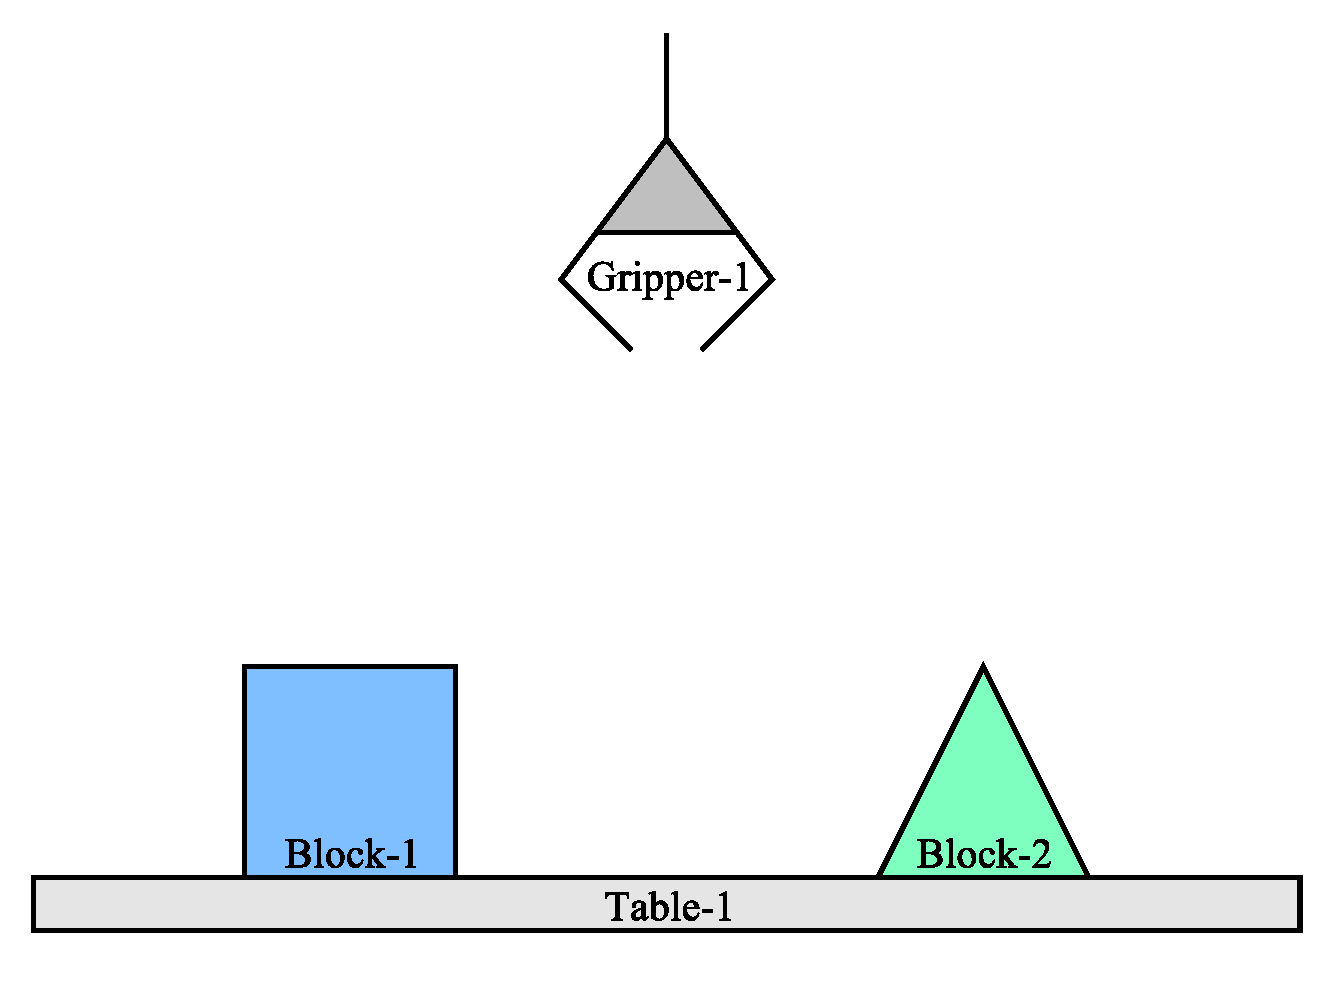
\includegraphics[width=6cm]{gfx/blocks_world_example-1}
  \caption[An example problem domain.]{An example problem domain.}
  \label{figure:an_example_problem_domain}
\end{wrapfigure}
has the goal of making a stack of two blocks.  The AI is now
confronted with the task of reasoning about how to get the physical
world into a state that matches this goal condition.  Specifically,
the AI must decide upon a plan of action, either creating a new plan
from scratch, or recalling a plan from memory that with some
modifications seems like it might work in this case.  When the AI
considers the plans that it knows, it remembers a plan that it has
been told will result in a stack of two blocks.  For example, the plan
shown in {\mbox{\autoref{table:a_plan_learned_from_being_told}}}
asserts that there is a stack of two blocks as its final operation.
If the AI were to recall this plan and execute it in the situation
shown in \autoref{figure:an_example_problem_domain}, the AI would
encounter an expectation failure at the final assertion of the
expected post-conditions of this plan.
{\mbox{\autoref{figure:failure_to_stack_cube_on_pyramid}}} shows how
executing this plan in this situation might fail to result in a stack
of two blocks: the pyramid does not support the cube, so the cube
falls off of the pyramid and onto the table.  In the case of a failure
of expectations, a refined hypothetical model of the physical world is
learned, so that the same planning mistake will never be made again.
\begin{wraptable}{l}{8cm}
\centering
\begin{tabular}{|rl|}
\hline
 1. & Move left.\\
 2. & Wait until a gripper is above a cube.\\
 3. & Reach and grab.\\
 4. & Wait until a gripper stops moving.\\
 5. & Move right.\\
 6. & Wait until a gripper is above a pyramid.\\
 7. & Drop and wait for block to fall.\\
 8. & Assert a cube is sitting on a pyramid.\\
\hline
\end{tabular}
\caption[A plan learned from ``being told''.]{A plan learned from
  ``being told''.}
\label{table:a_plan_learned_from_being_told}
\end{wraptable}
In my AI, learning a new physical model of the world amounts to
relearning the hypotheses for the expected transframes that result
from executing different physical actions, leading from one collection
of physical situation type events to another.  In this case, the AI
learns many new refined hypotheses about the physical world.  For
example, the AI learns that executing the action of moving to the left
until a cube is below the gripper results in a cube being below the
gripper.  Of course, this may not generally be true, but the AI's
physical action hypotheses are refined in light of this added
experiential knowledge that predicts this change given the specific
preconditions.  The AI still retains many hypotheses that leave room
for the possibility that executing this action in other preconditions
may or may not result in this specific change.  For example, at this
point, the AI has no experience executing this action when there is
not a block to the left of the gripper.  In that case, the AI cannot
be sure that this action will result in a block being below the
gripper, and this uncertainty is represented in the hypothesis space
of the AI's concept learning algorithm.

In addition to learning a refined hypothetical model of the physical
world, the AI also learns a better model of how to control its
planning machine that chose this plan for some reason and decided to
execute it.  In other words, not only has the AI failed to act
physically but also the AI has failed in thinking about its plans.
The AI decided to execute a plan that ended up failing.  Because the
AI has a reflective learning algorithm, it has the additional ability
to learn a better model of the planning process itself---the planning
process that selected this plan, imagined its physical effects, and
decided to execute it.

Deliberative planning processes are plans of the reflective
metacognitive reasoning layer.  The reflective layer contains a
metacognitive planning machine that creates, reasons about, and
executes plans for how to control the deliberative planning machine.
Thus, the AI has two layers of planners: one planner that learns about
physical processes and another planner that learns about planning
processes.  A plan for physical action is manipulated by resources in
the deliberative layer, while a plan for deliberative action is
manipulated by resources in the reflective layer.

In this example, the goal of the reflective planning machine is to
attempt to avoid plan execution failures, while executing plans that
are hypothesized to accomplish physical goals.  The plan executed in
the deliberative planner resulted in a physical expectation failure.
The plan attempted to assert that a cube is supported by a pyramid,
which was not true at the point when the assertion was executed in the
deliberative planning machine.  When a plan encounters a specific type
of failure, properties of the failure event are represented as a
failure object that is associated with the plan object that failed.
As seen by the reflective layer, the deliberative failure knowledge is
related to the plan in a way that is analogous to the way that the
deliberative layer sees a physical block sitting on another physical
block.  The deliberative layer learns how to control relationships
between physical objects, while the reflective layer learns how to
control relationships between deliberative objects, such
\begin{figure}{h}
  \centering
  \begin{tabular}{p{5cm}p{5cm}}
    1. 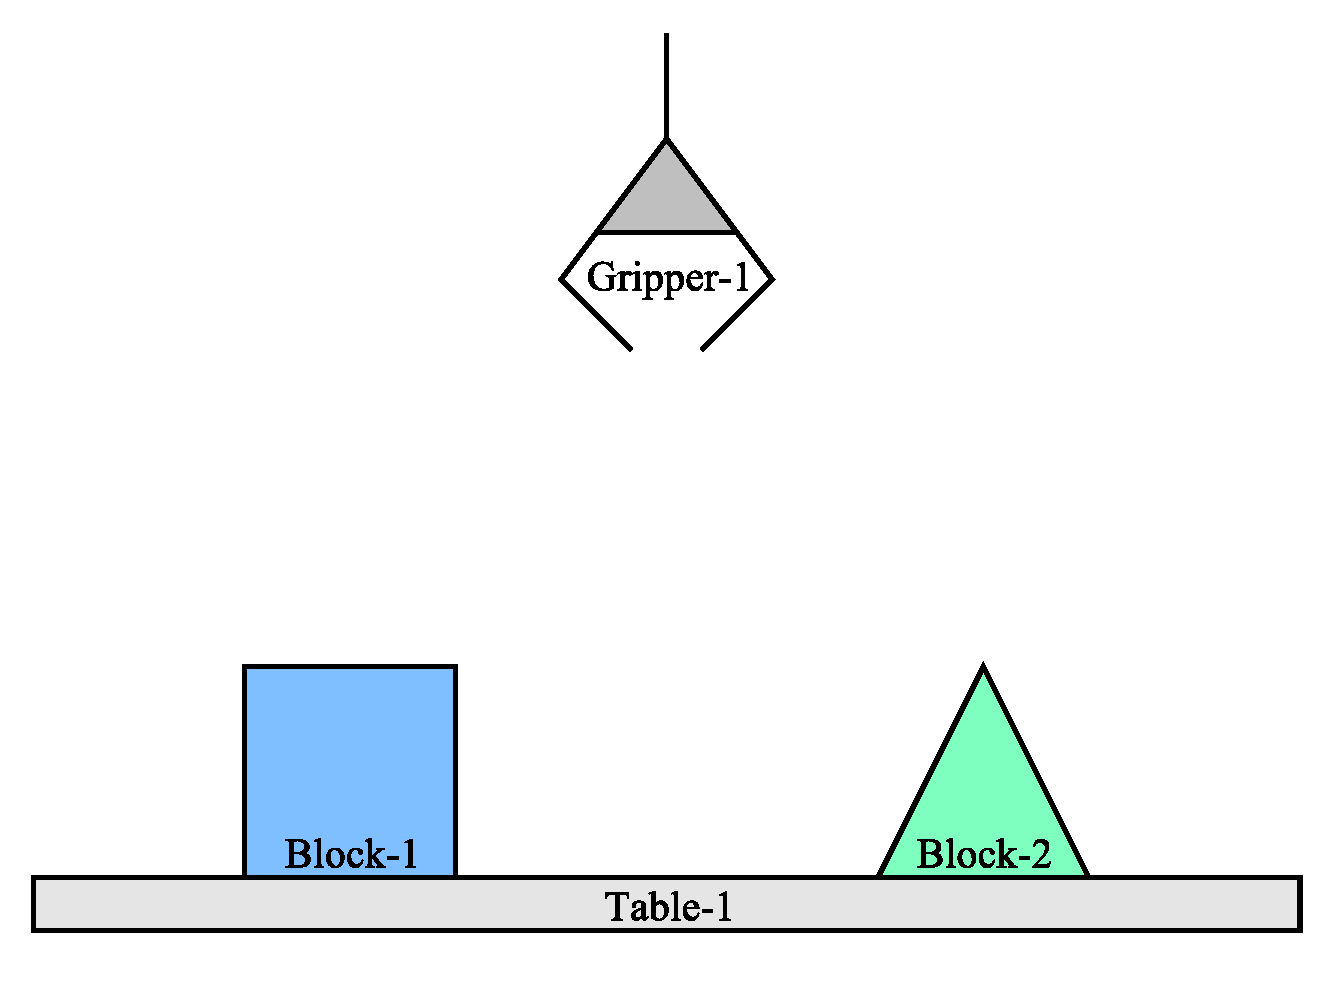
\includegraphics[width=5cm]{gfx/blocks_world_example-1}  & 2. 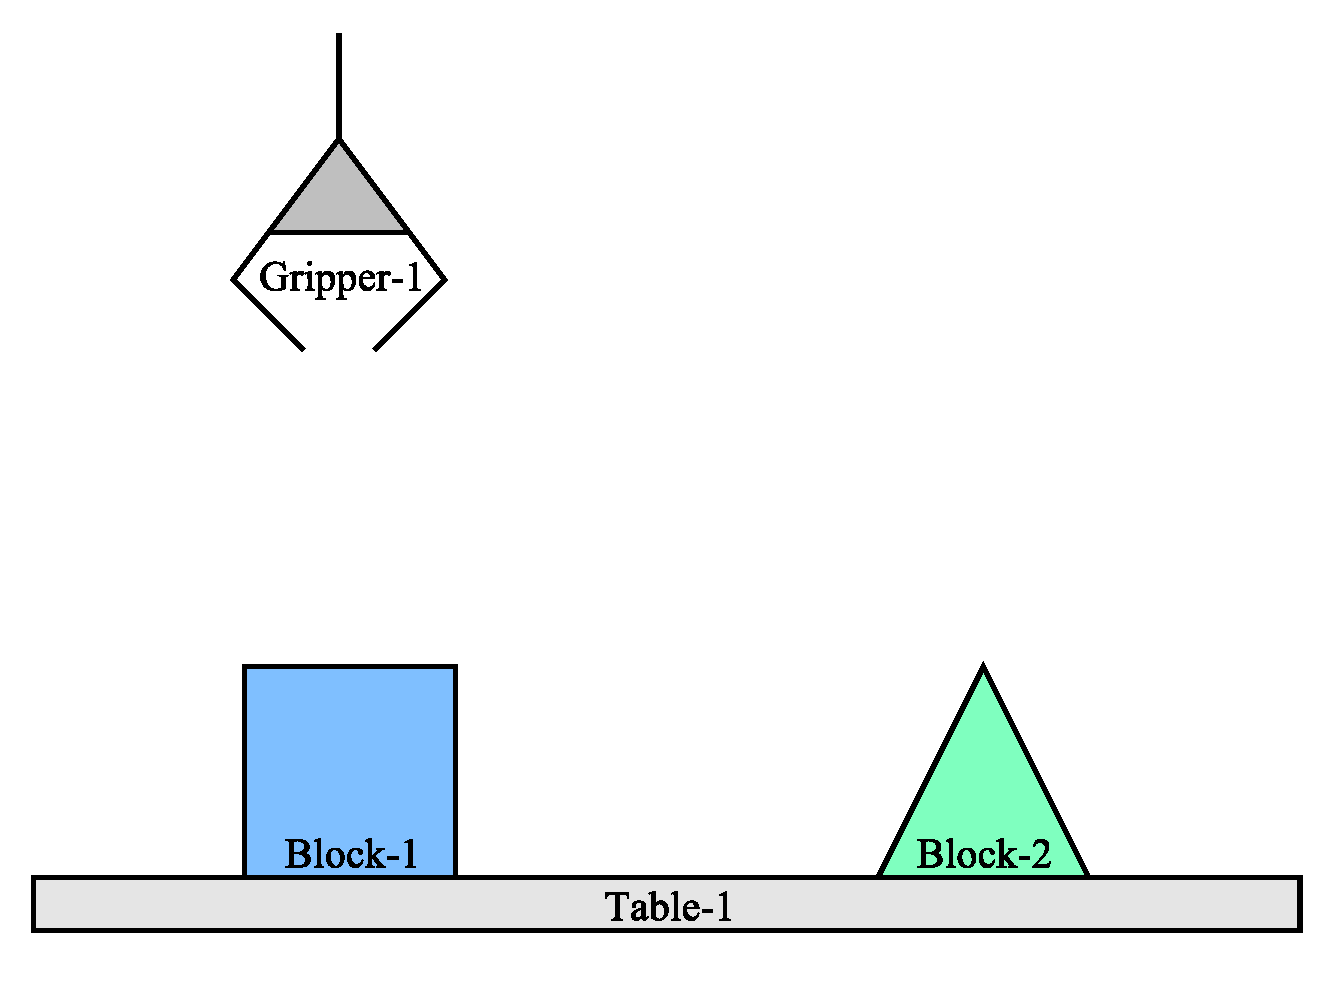
\includegraphics[width=5cm]{gfx/blocks_world_example-2} \\
    3. 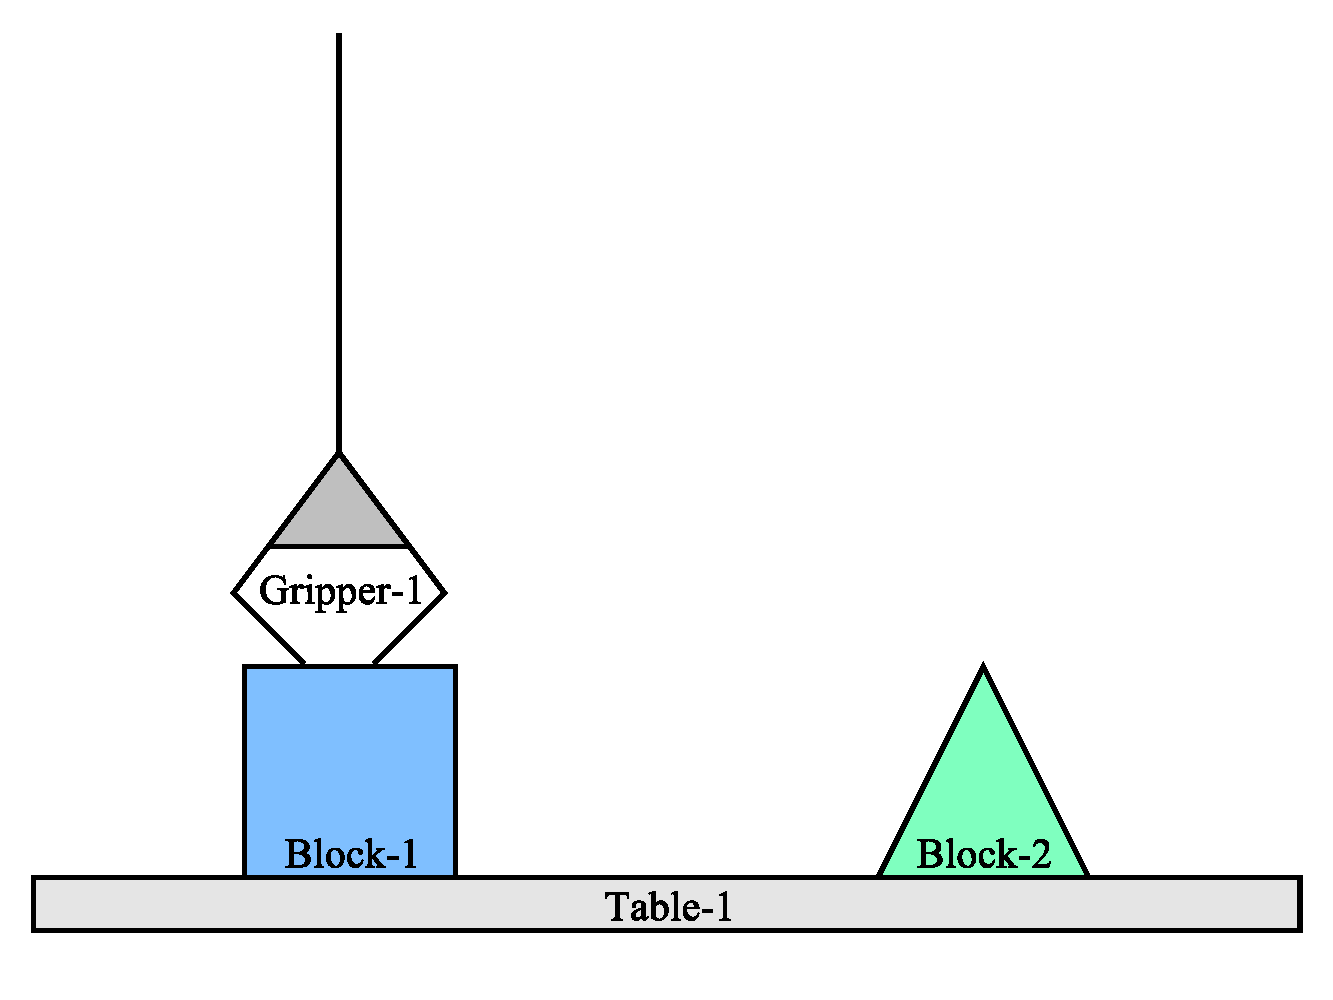
\includegraphics[width=5cm]{gfx/blocks_world_example-3}  & 4. 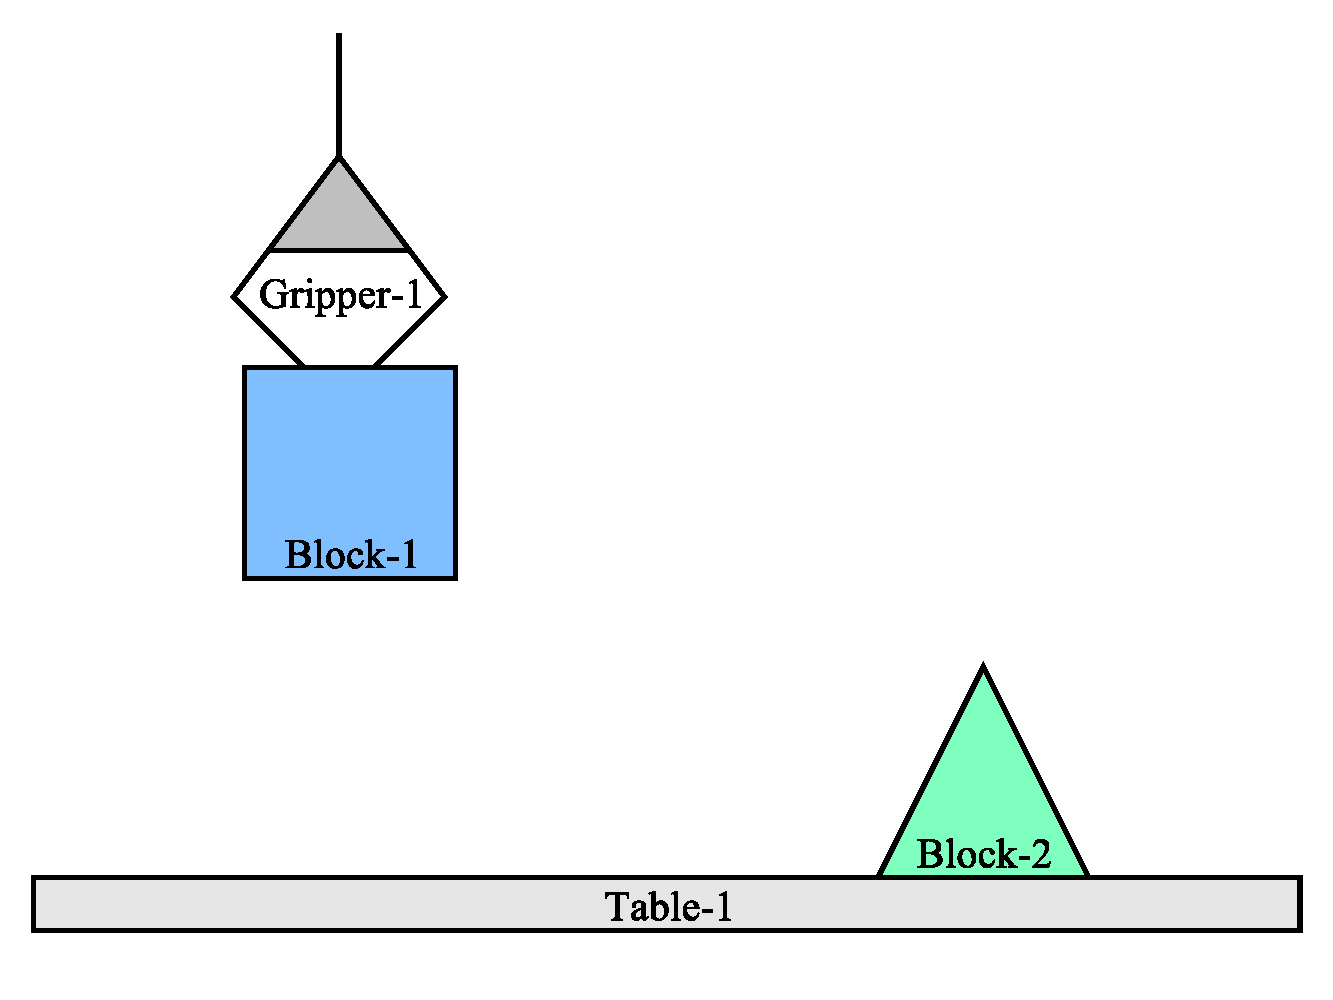
\includegraphics[width=5cm]{gfx/blocks_world_example-4} \\
    5. 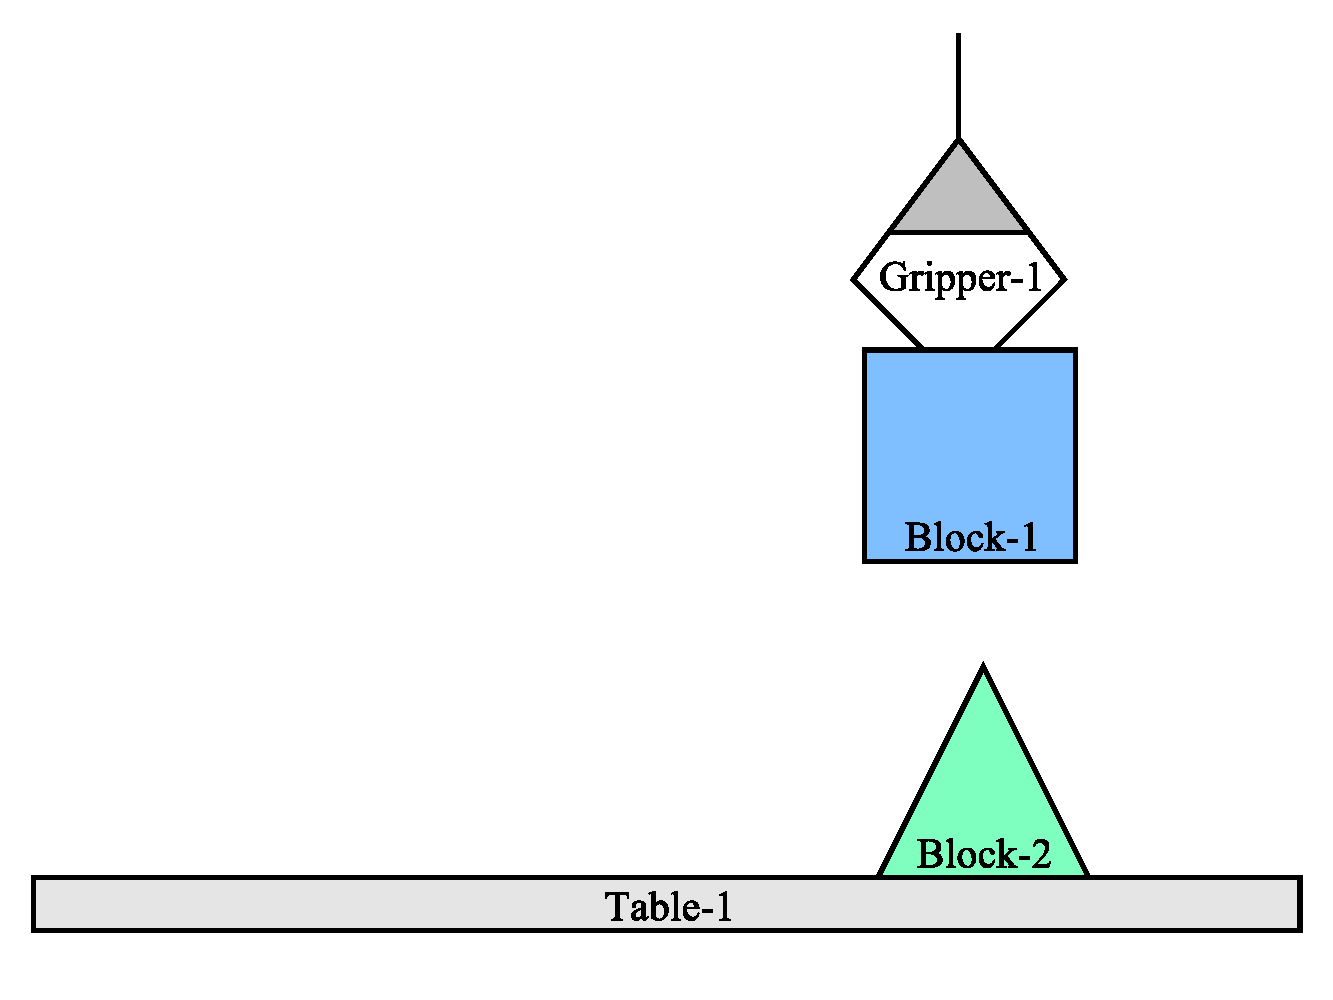
\includegraphics[width=5cm]{gfx/blocks_world_example-5}  & 6. 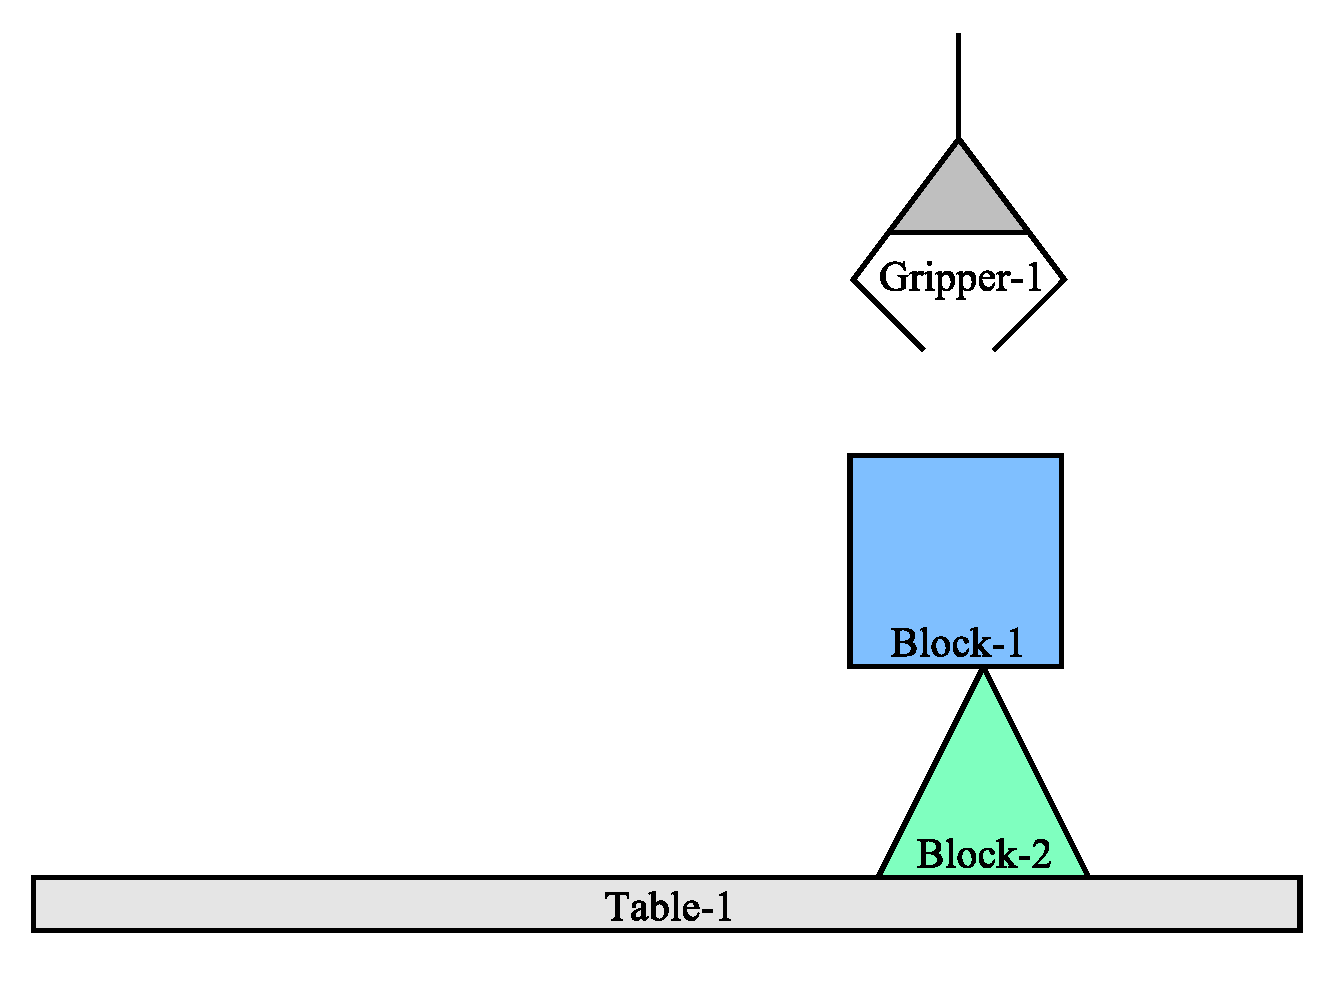
\includegraphics[width=5cm]{gfx/blocks_world_example-6} \\
    7. 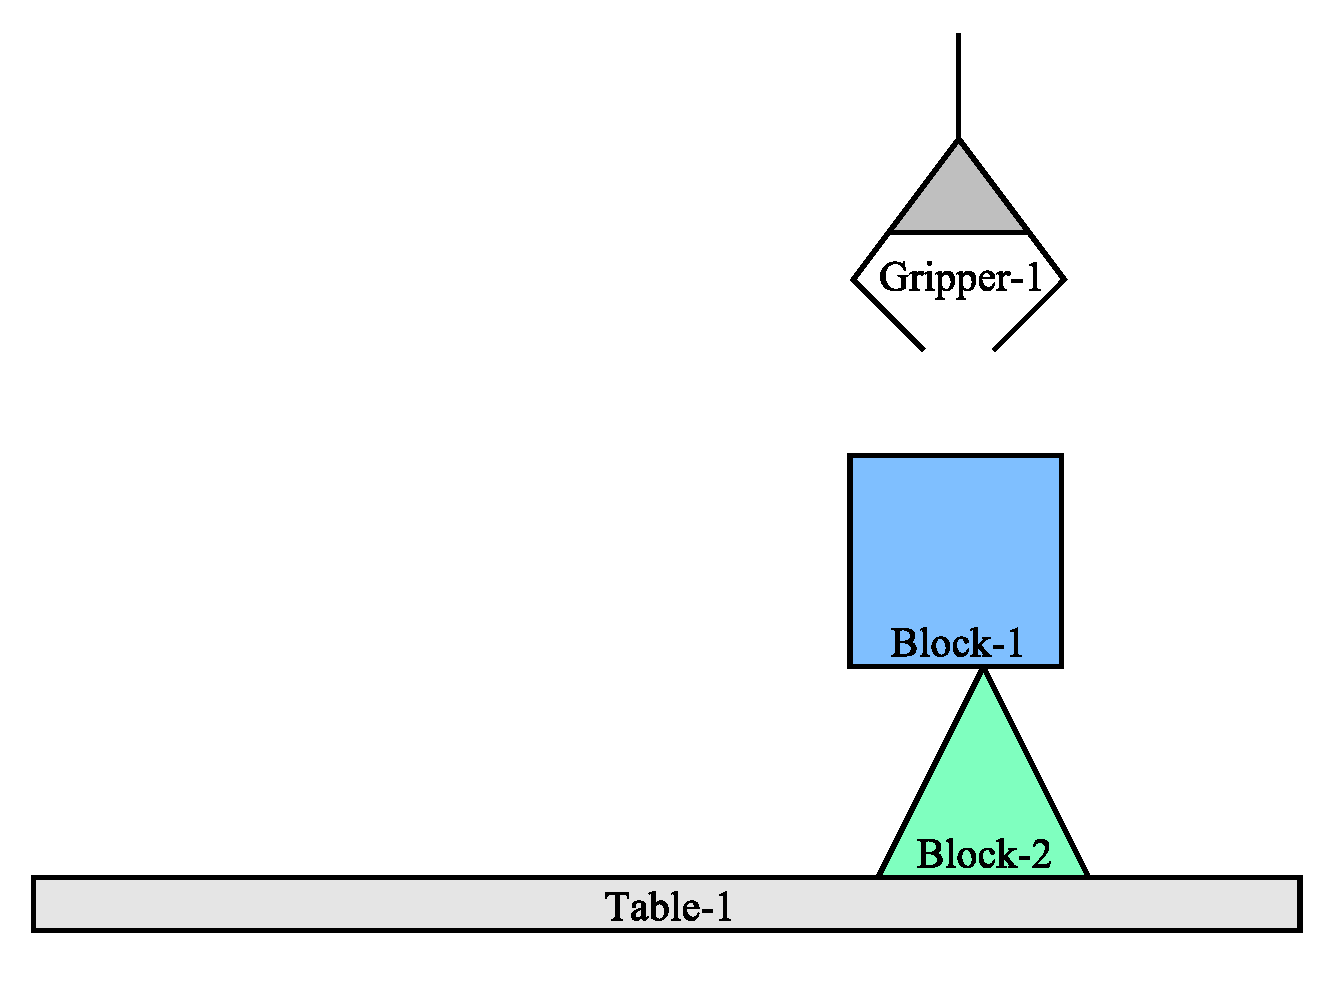
\includegraphics[width=5cm]{gfx/blocks_world_example-7}  & 8. 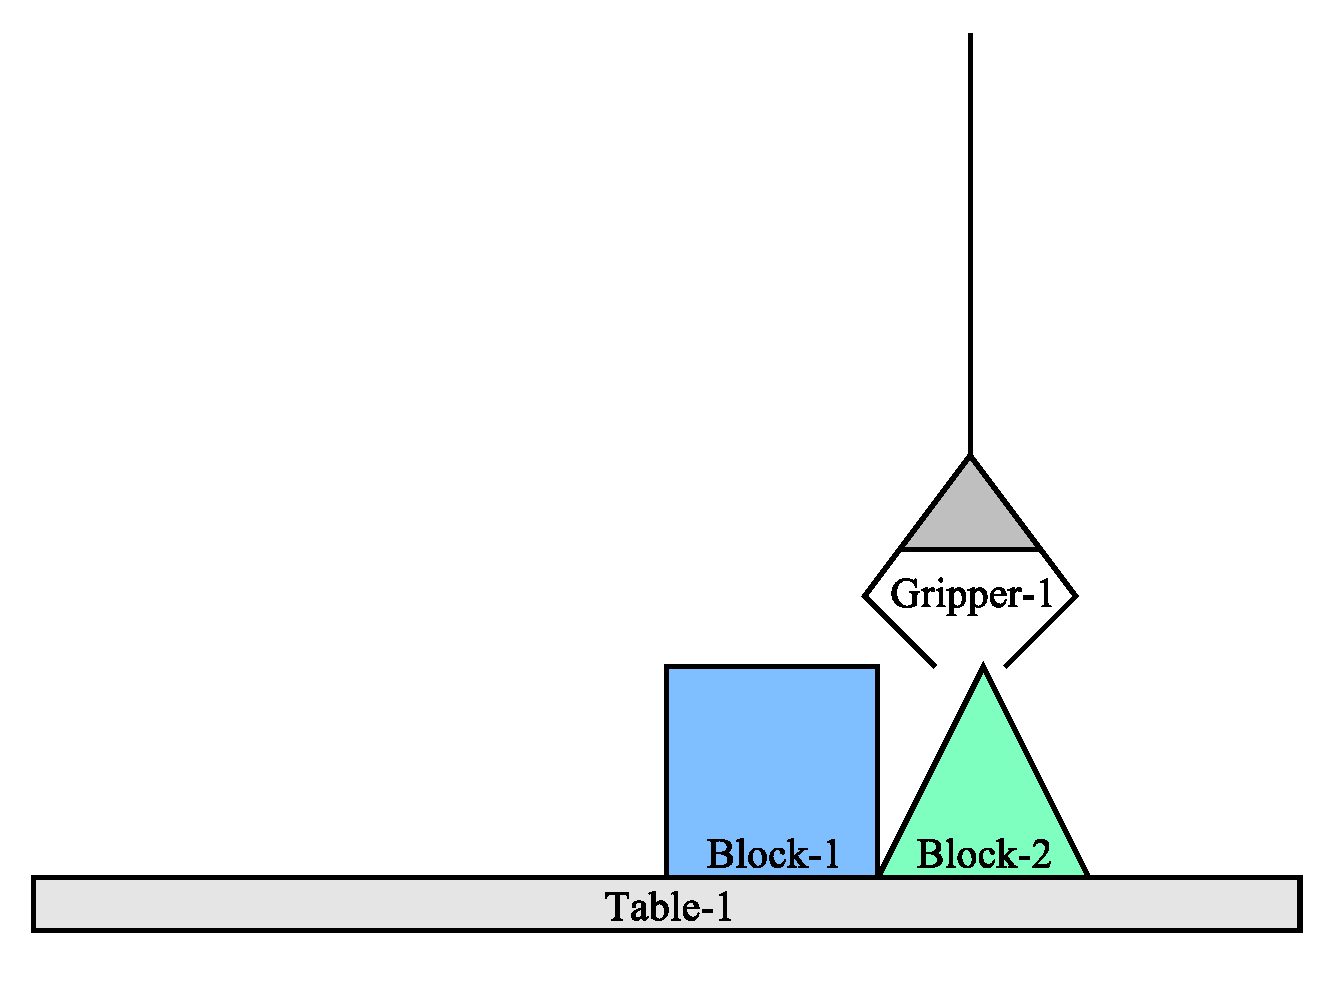
\includegraphics[width=5cm]{gfx/blocks_world_example-8}
  \end{tabular}
  \caption[An example of an expectation failure.]{An example of an
    expectation failure.  A plan is executed that asserts that a
    post-condition must be a stack of a cube sitting on a pyramid,
    but when the plan finishes executing this assertion fails.}
  \label{figure:failure_to_stack_cube_on_pyramid}
\end{figure}
as the deliberative planning machine, plans, hypotheses, and execution
failures.

The reflective layer learns models of how deliberative actions change
the types of knowledge relationships between objects in the
deliberative layer.  The reflective planning machine attempts to
accomplish deliberative type knowledge goals computed from this
deliberative knowledge.  Here is a list of deliberative type knowledge
that the reflective layer can know about the objects in the
deliberative layer:
\begin{itemize}
\item A plan that asserts that a cube is sitting on a pyramid is
  under the focus of the deliberative planning machine.
\item A plan that has had an expectation failure is being executed by
  the deliberative planning machine.
\item There is no plan currently executing in the deliberative
  planning machine.
\item There is a plan to drop a block that you are holding before
  reaching and grabbing.
\item The deliberative planning machine is focused on a plan to move
  to the left while concurrently moving to the right.
\end{itemize}
These types of states are learned in the reflective layer by
processing a procedurally reflective event stream generated by the
deliberative layer planning processes.  These types of states are
potential goals, preconditions, and effects in the reflective planning
machine that models how deliberative actions effect the types of
states in the deliberative planning-machine knowledge.  Reflective
hypotheses about the deliberative layer are learned in terms of these
types of states.  The reflective layer learns hypotheses for
predicting types of plan execution failure knowledge from other
deliberative types of knowledge preconditions.

In the example, executing the plan that the deliberative planner is
focused on is hypothesized to result in a plan having an expectation
failure event.  The reflectively planned execution of the deliberative
execution of the plan is processed concurrently with the deliberative
planning machine operations, slightly behind the times, not
necessarily slowing down the deliberative planning resources.  The
reflective layer induces deliberative types of knowledge from this
reflectively reconstructed deliberative planning machine knowledge
base.  The preconditions and effects of the deliberative execution
actions are learned from the types of this reflective reconstruction,
learning to predict, in terms of types of knowledge, the effects of
planning actions on plans in general.  In the example, these types of
knowledge include: ``The plan currently under focus contains an
assertion that a cube must be stacked on a pyramid.''  The AI refines
many of its hypotheses given this limited experience of failure,
retaining the hypothesis that executing the plan under focus might
result in failure due to the plan's assertion that a cube is sitting
on a pyramid.

{\mbox{\autoref{figure:implemented_example_learning_storyboard}}}
shows an example of how reflectively learning about the deliberative
planning machine can lead to the successful achievement of a physical
goal.  In this example, the reflective layer infers the results of
executing plans and tries to predict their failure based on the
structure of the plan and its relationship to other deliberative
knowledge, such as different types of failure events.
{\mbox{\autoref{table:a_metacognitive_plan_learned_from_being_told}}}
shows an example metacognitive plan that the reflective layer is
executing in order to control the deliberative planning machine.
Based on these planned resource activations from the reflective layer,
the deliberative layer recalls a plan from memory that it has ``been
told'' but does not have experience executing.
\begin{wraptable}{l}{8cm}
\centering
\begin{tabular}{|rl|}
\hline
 1. & While no plans for goal, repeat 2--7.\\
 2. & ~~Forget all imagined events.\\
 3. & ~~Set imagine time to be now.\\
 4. & ~~Imagine current situation.\\
 5. & ~~Recall plan from memory.\\
 6. & ~~Imagine executing plan in focus.\\
 7. & ~~Check goals in imagination.\\
 8. & Recall plan for goal.\\
 9. & Execute plan in focus.\\
\hline
\end{tabular}
\caption[A metacognitive plan in the reflective layer learned from
  ``being told''.]{A metacognitive plan in the reflective layer
  learned from ``being told''.}
\label{table:a_metacognitive_plan_learned_from_being_told}
\end{wraptable}
The reflective layer imagines executing the plan for deliberation in
terms of the planning machine of the deliberative layer.  The
reflective layer imagination does not include physical effects of
physical actions.  The reflective layer only learns from and predicts
the types of knowledge in the deliberative layer, such as the
properties and relationships between the planning machine, plans, and
failure events.  Because of the AI's lack of experience, the
reflective layer does not infer that this plan for physical action
will lead to a failure in the deliberative planning machine based on
its structure.  Further, because of the AI's inexperience with
physical actions, when it reflectively decides to execute this
deliberative plan, it deliberatively infers that this plan will
actually create a stack of two blocks.  Both of these forms of
ignorance are corrected when the AI attempts to execute the chosen
plan.  Not only is a new model of the physical world learned but also
a new model of the deliberative planning machine is learned by the
reflective layer.  In this way, the failure to predict the effects of
physical actions can also be considered a failure to predict the
effects of deliberative actions.  In other words, the reflective layer
made a mistake in controlling the planning machine by having it
execute a plan that ended up failing.  In general, the reflective goal
to control the deliberative machine to avoid execution failures is not
absolutely necessary.  In other situations it may be desirable for
physical failures to occur.  For example, if the AI is performing an
experiment or ``playing'' in a physical domain, it may be desirable to
fail in order to accomplish knowledge level goals.  In this example,
the reflective planner has a negative goal, which is: ``Avoid
Deliberative-Planner-1 just having had an execution failure.''
\begin{figure}
\centering
\begin{tabular}{p{3.5cm}p{3.5cm}p{3.5cm}}
1. 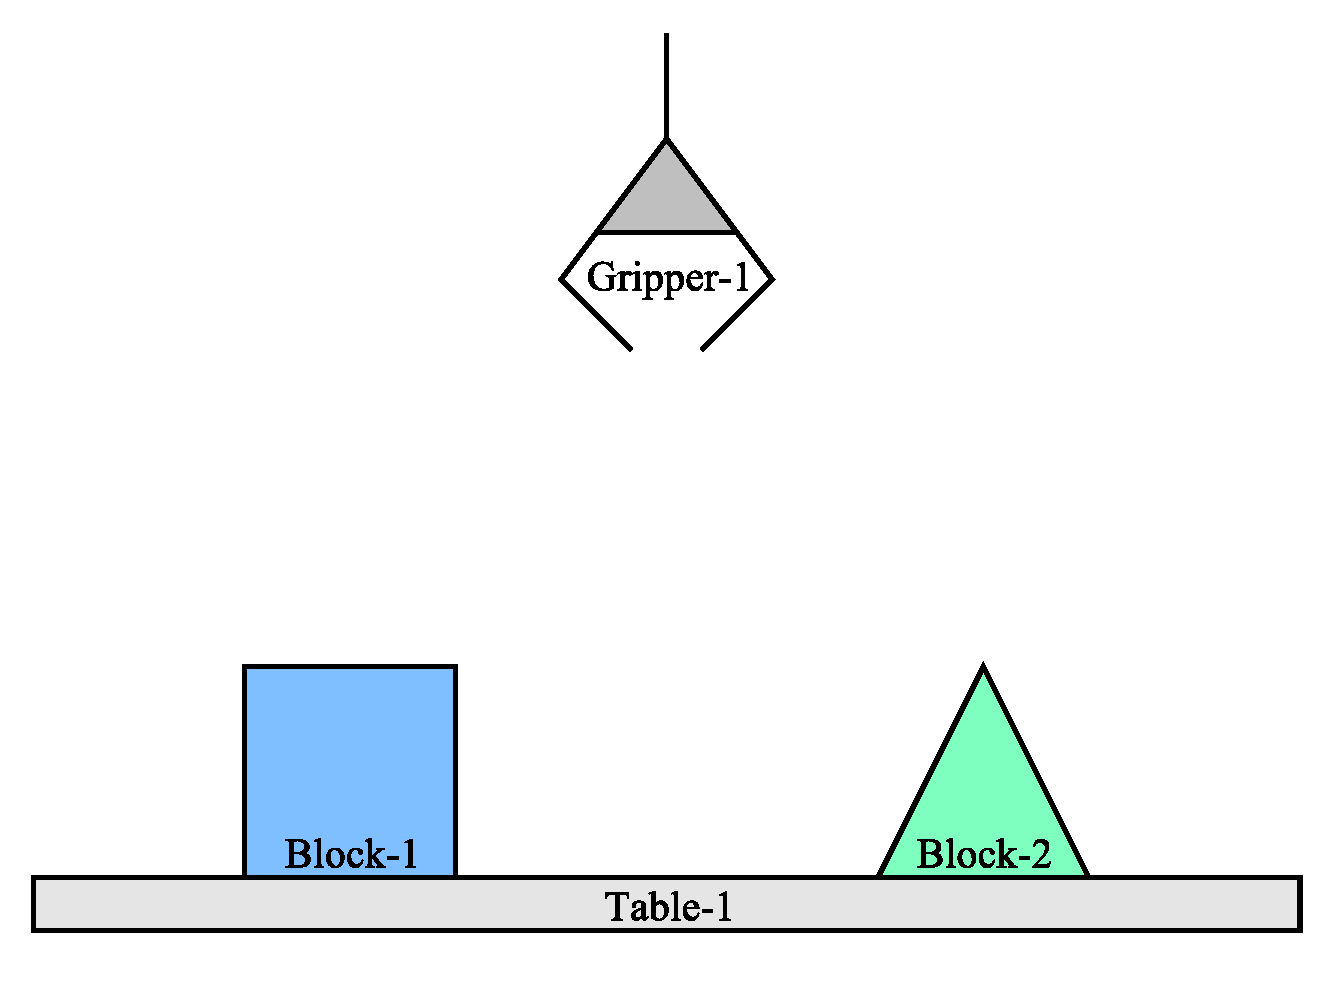
\includegraphics[width=3.5cm]{gfx/blocks_world_example-1}  & 2. 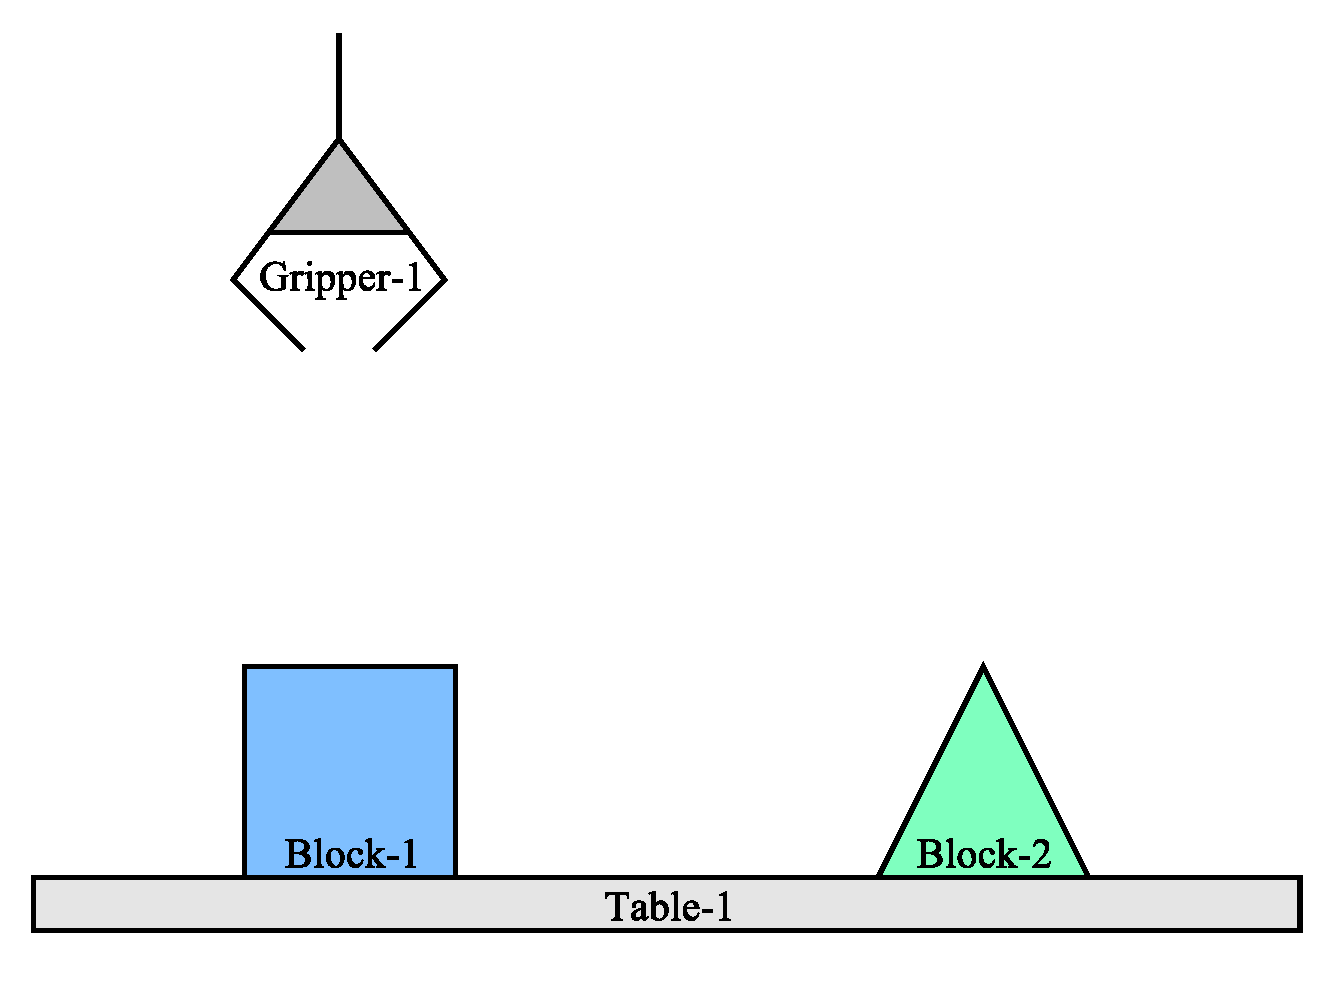
\includegraphics[width=3.5cm]{gfx/blocks_world_example-2}  & 3. 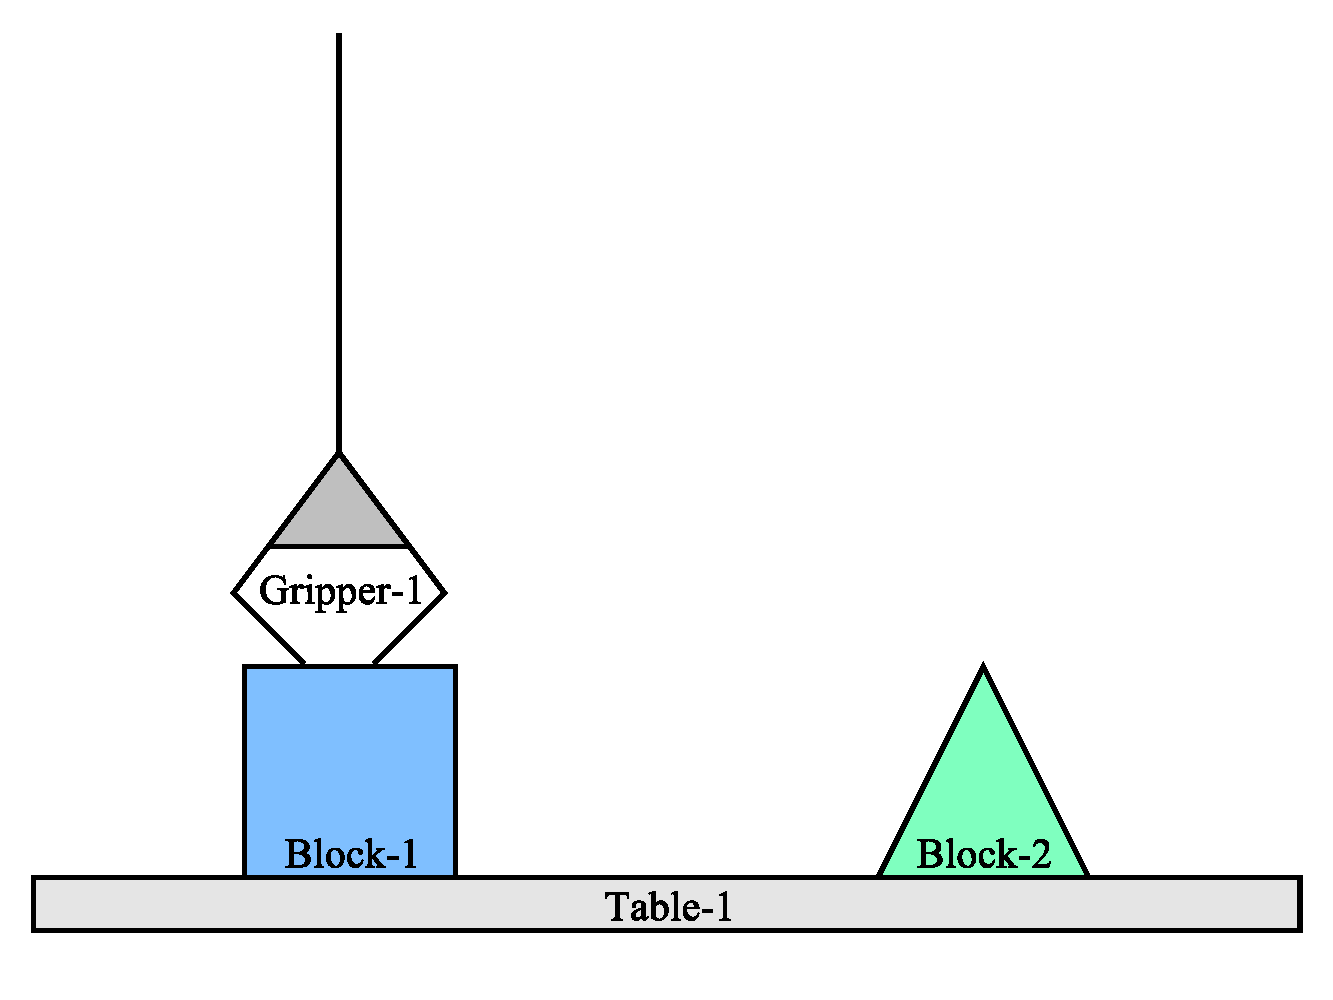
\includegraphics[width=3.5cm]{gfx/blocks_world_example-3} \\
4. 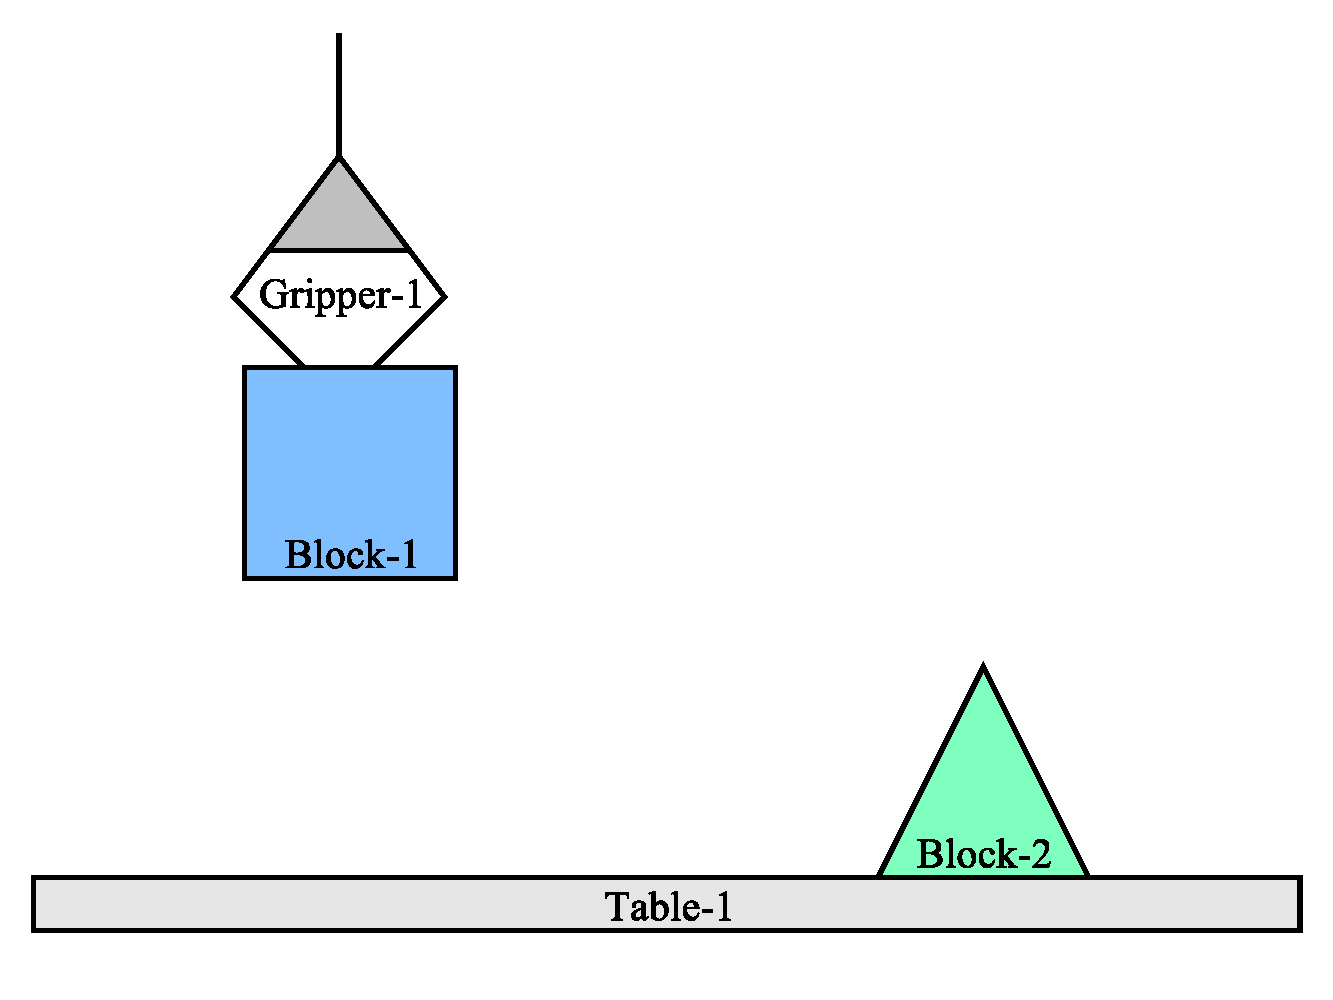
\includegraphics[width=3.5cm]{gfx/blocks_world_example-4}  & 5. 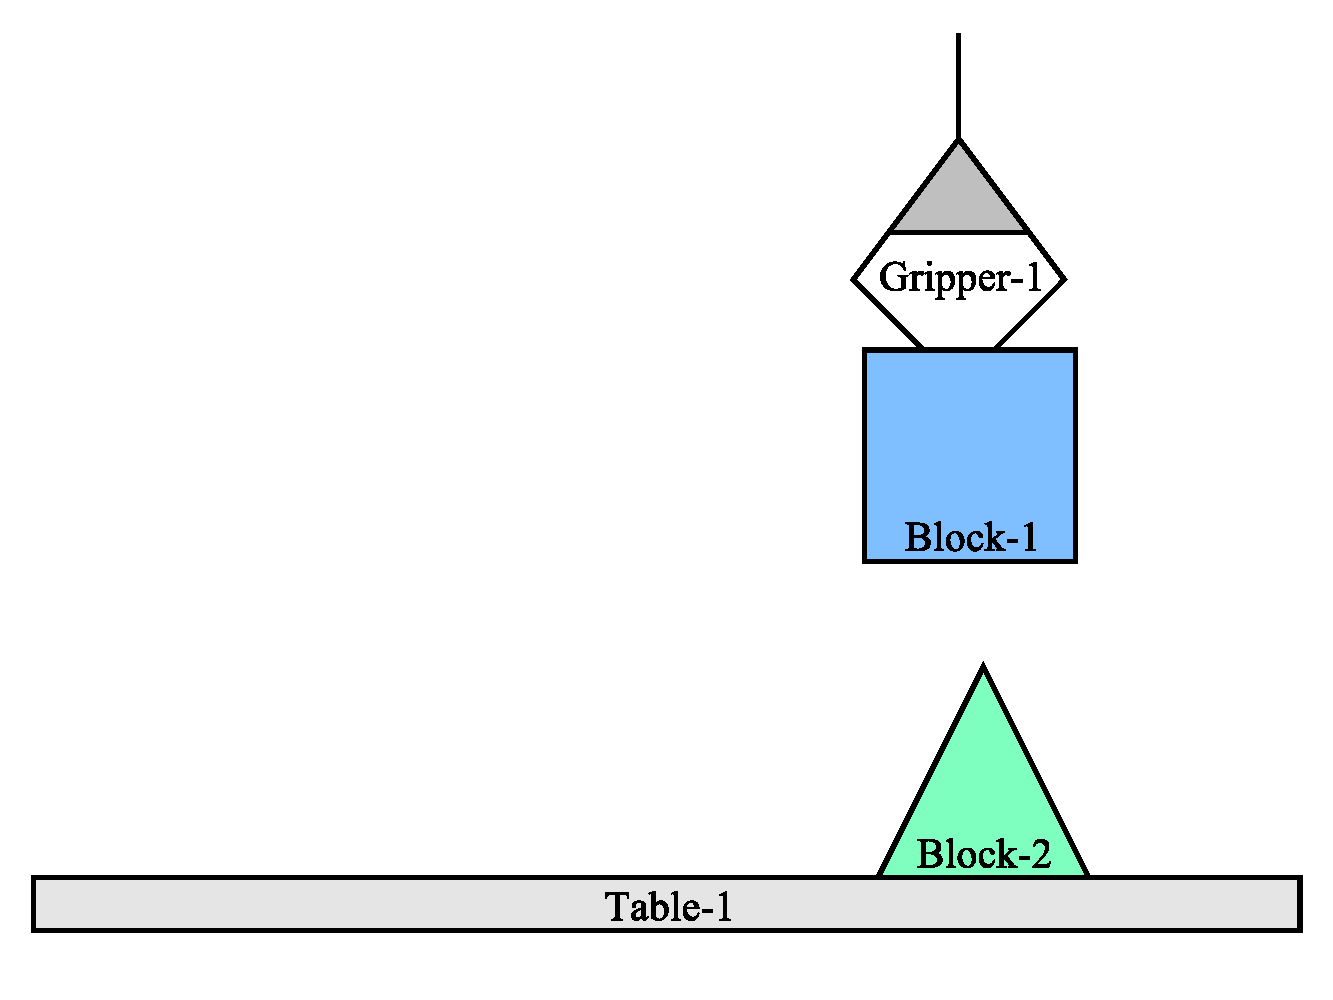
\includegraphics[width=3.5cm]{gfx/blocks_world_example-5}  & 6. 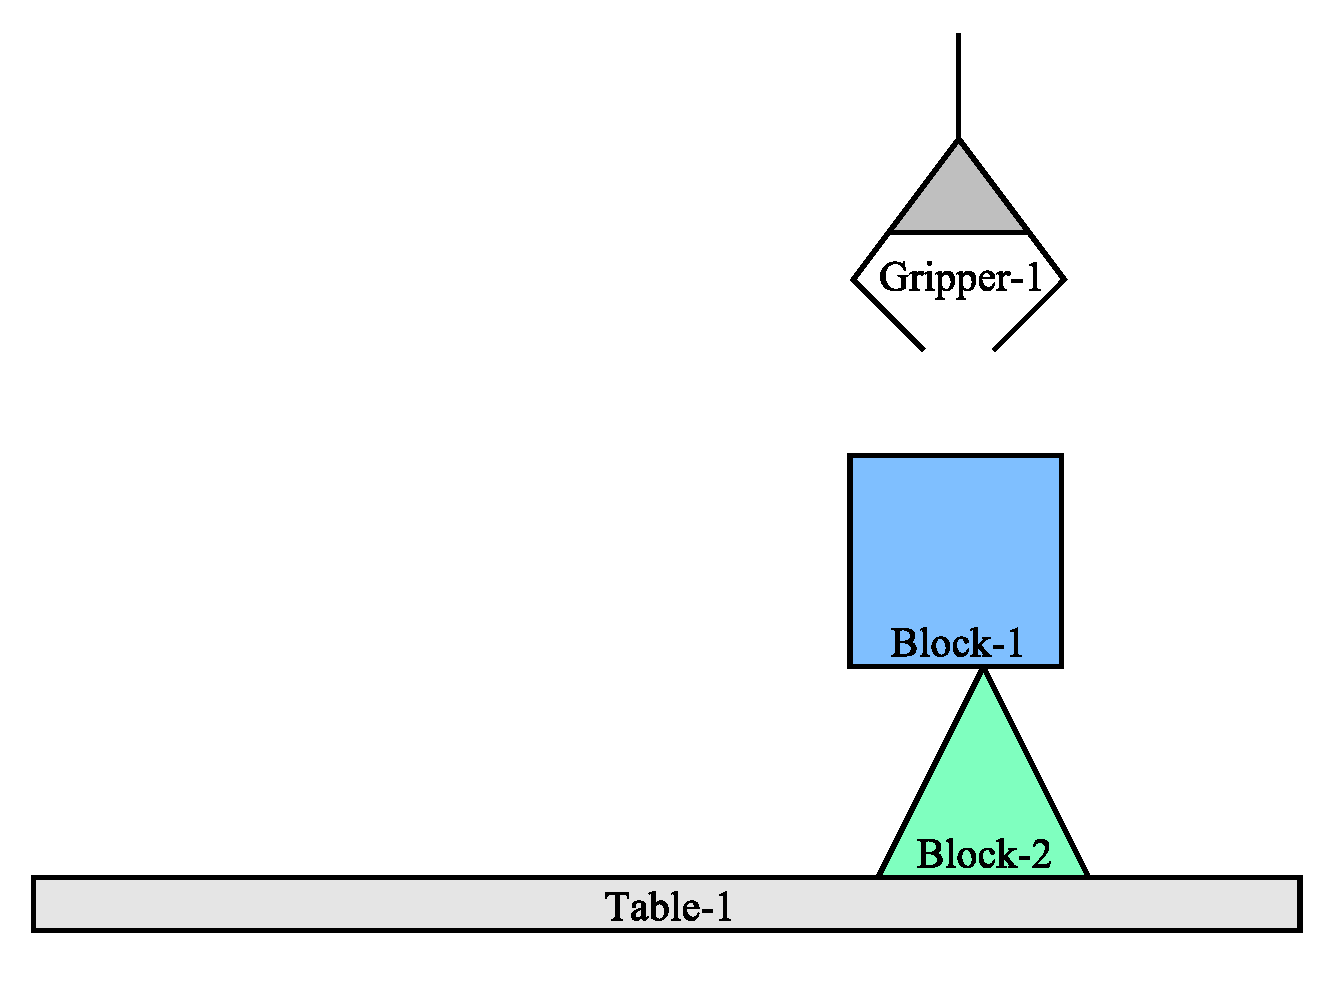
\includegraphics[width=3.5cm]{gfx/blocks_world_example-6} \\
7. 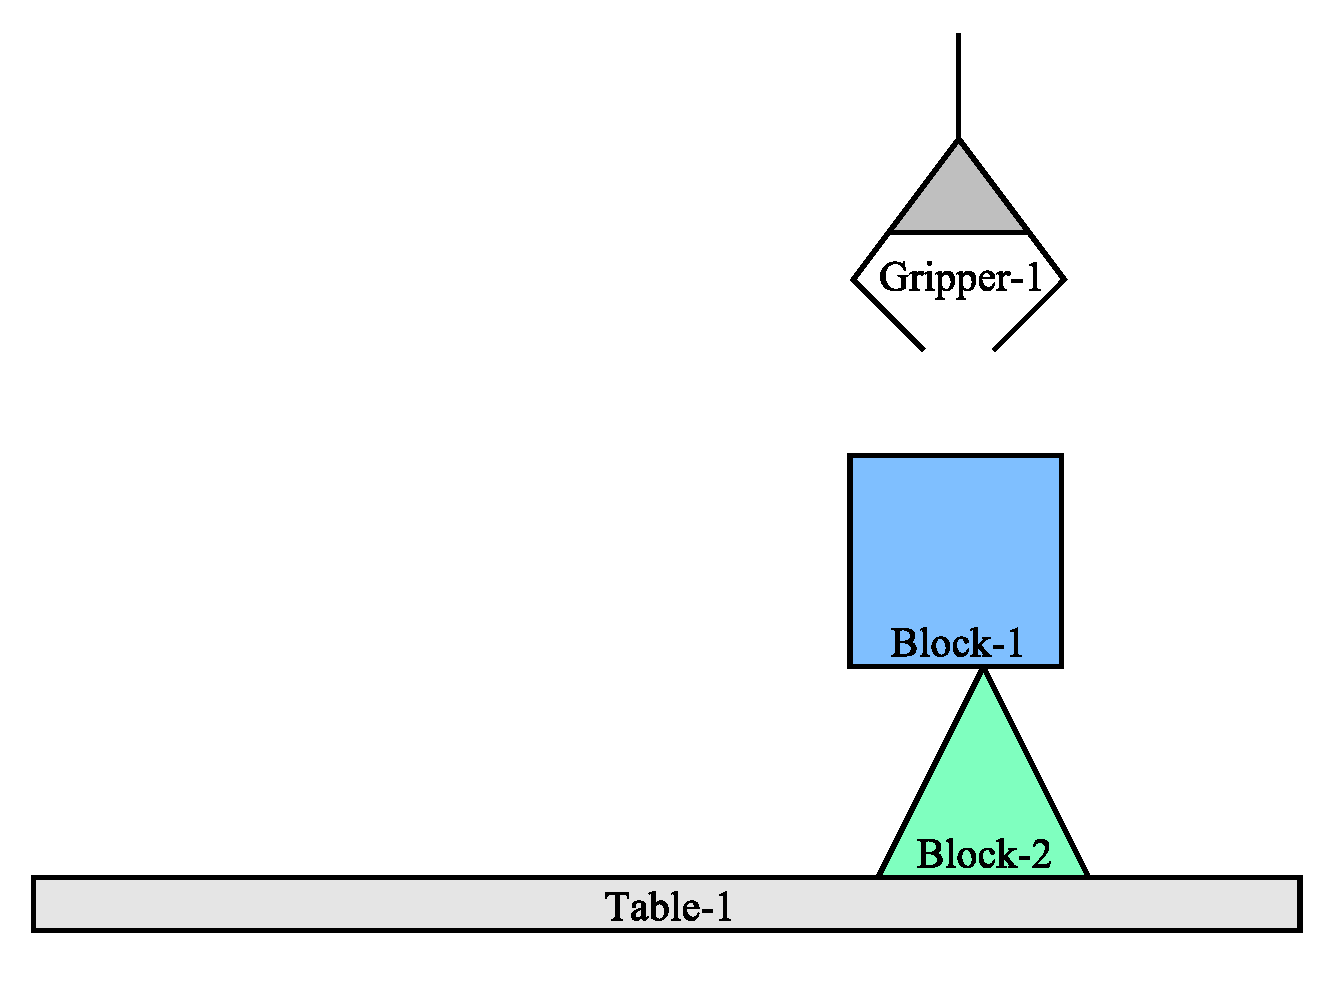
\includegraphics[width=3.5cm]{gfx/blocks_world_example-7}  & 8. 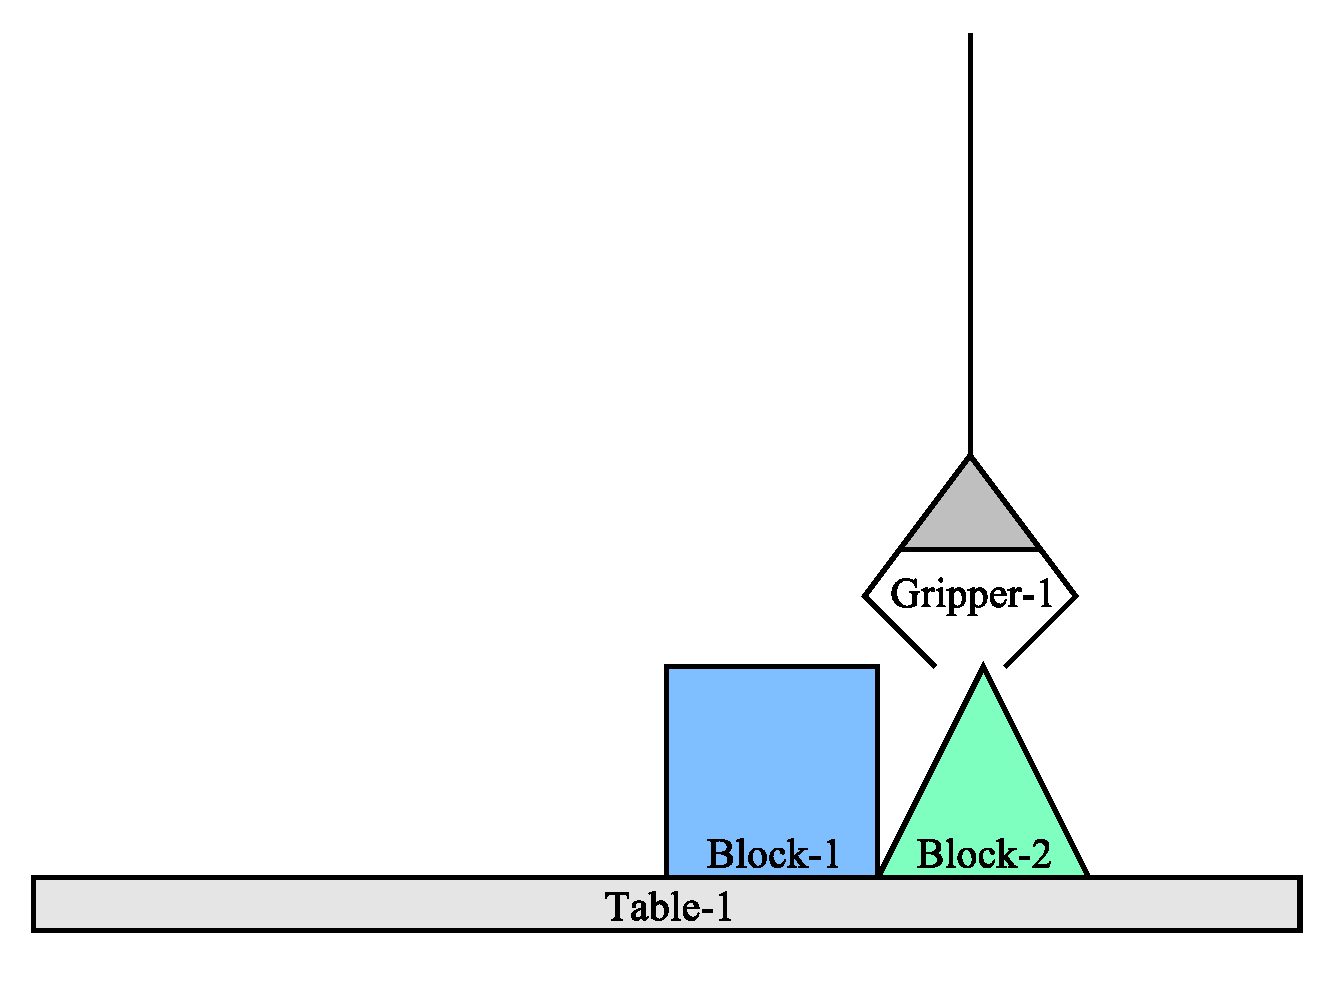
\includegraphics[width=3.5cm]{gfx/blocks_world_example-8}  & 9. 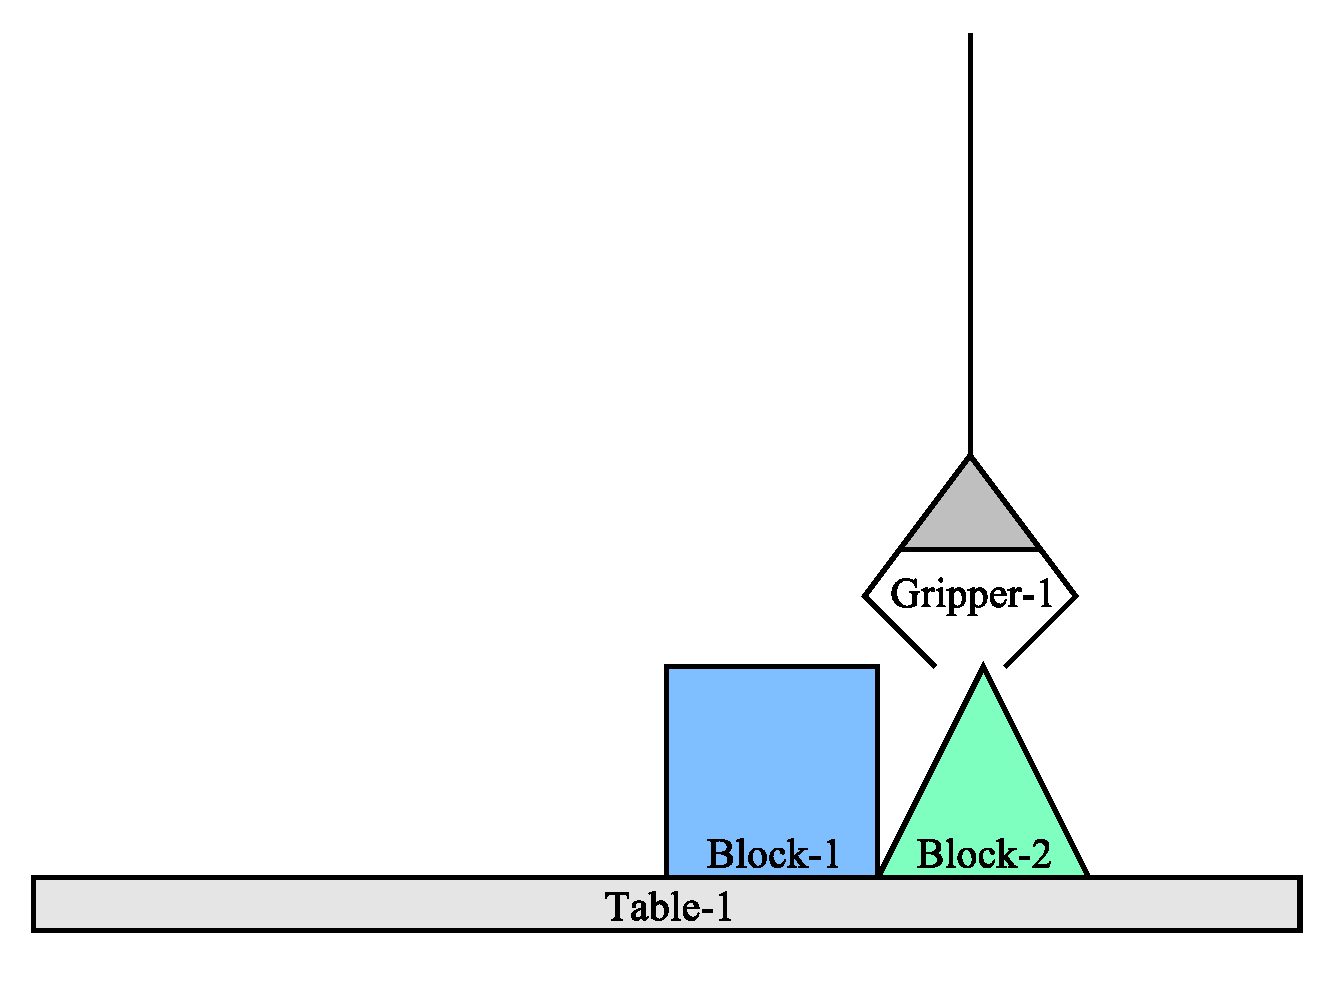
\includegraphics[width=3.5cm]{gfx/blocks_world_example-9} \\
10. 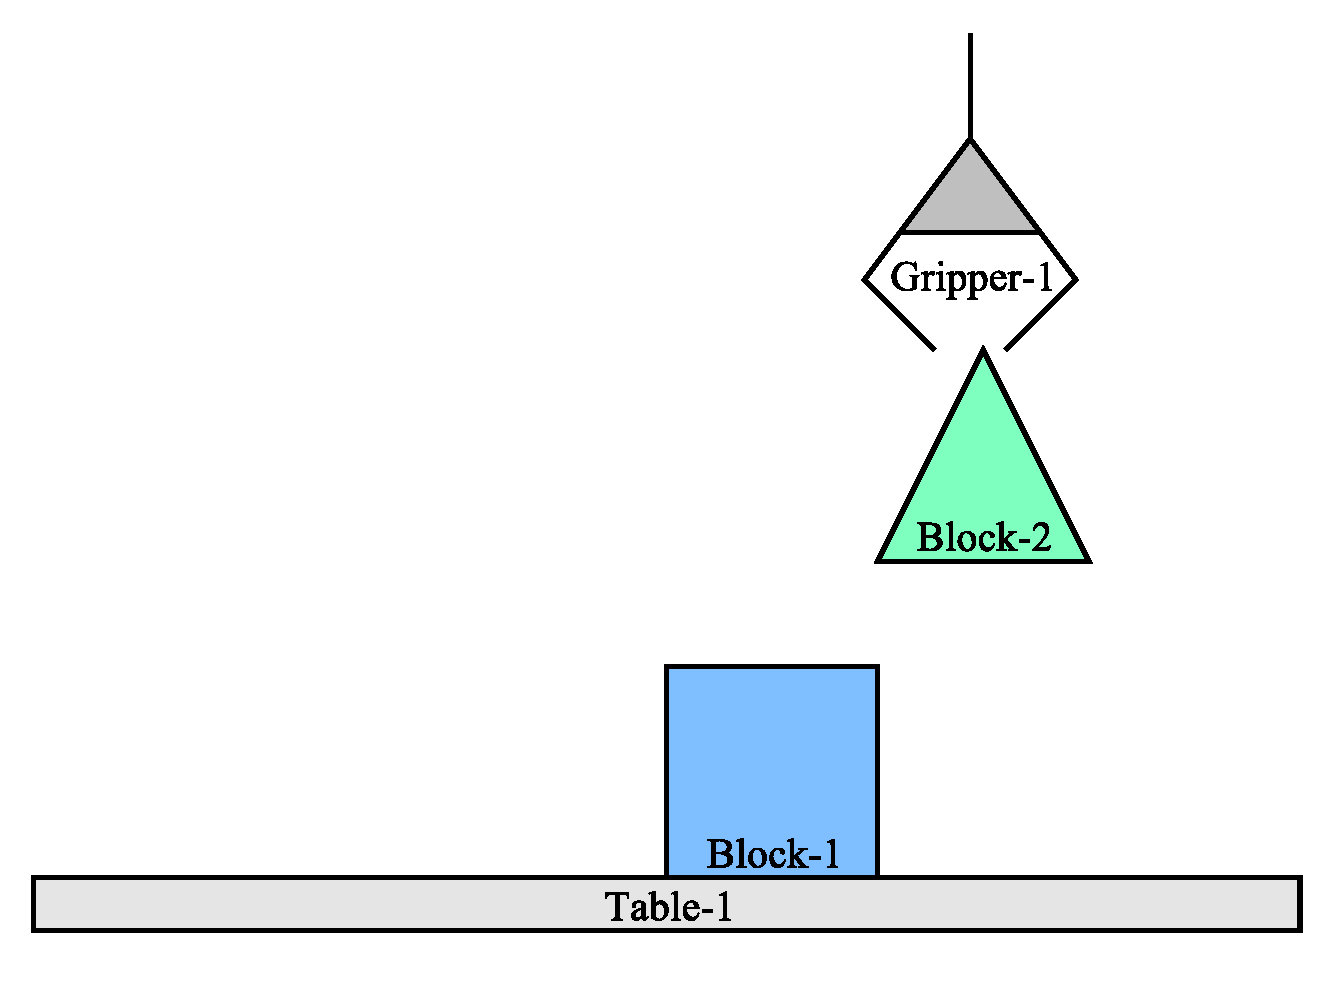
\includegraphics[width=3.5cm]{gfx/blocks_world_example-10} & 11. 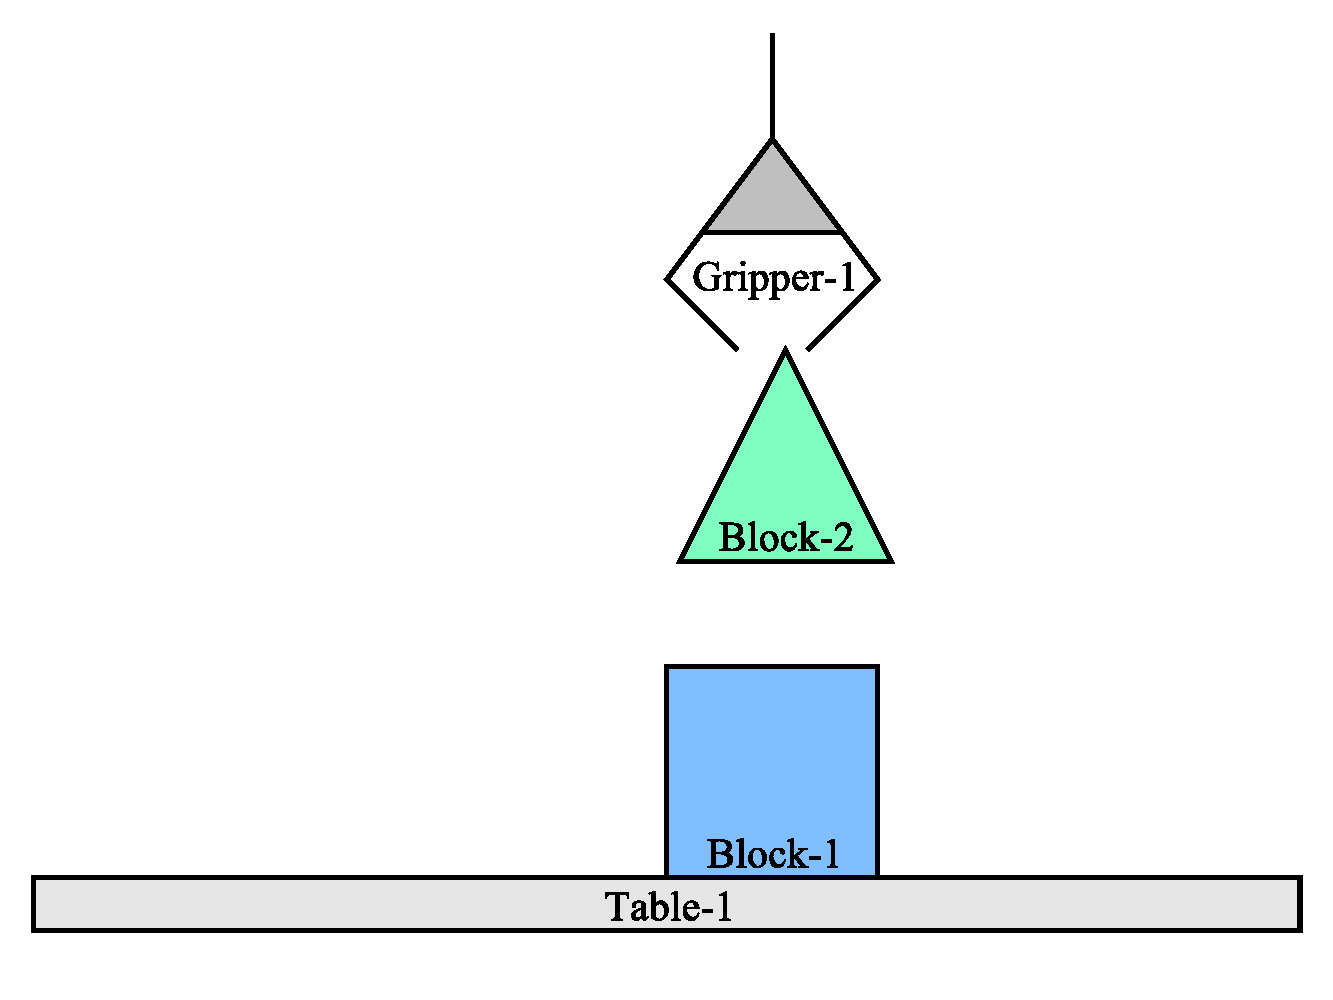
\includegraphics[width=3.5cm]{gfx/blocks_world_example-11} & 12. 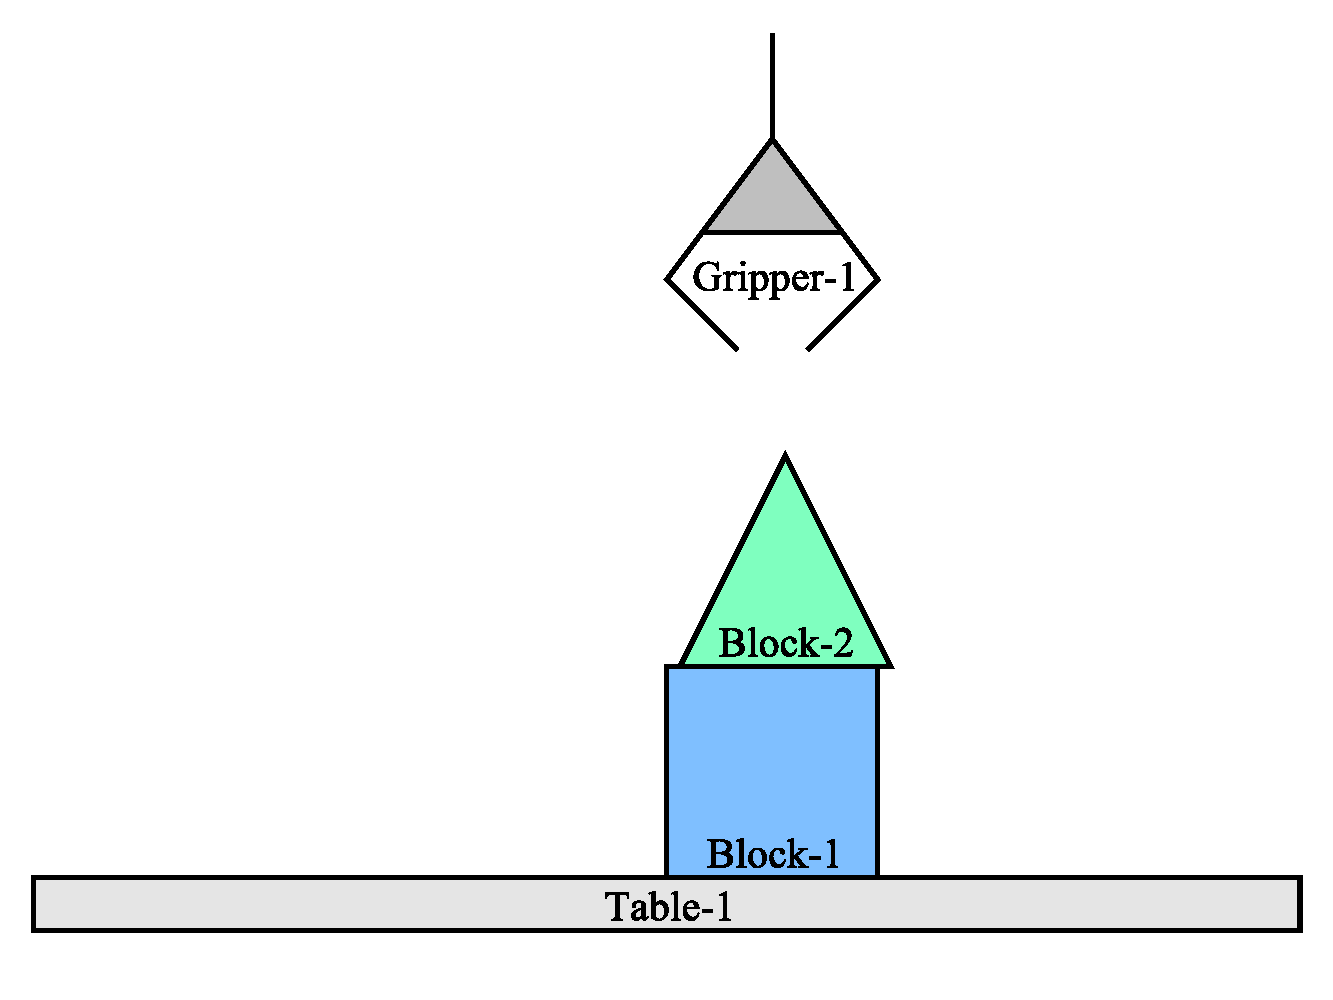
\includegraphics[width=3.5cm]{gfx/blocks_world_example-12}
\end{tabular}
\caption[Adaptation due to reflectively learning how to
  deliberate.]{Adaptation due to reflectively learning how to
  deliberate.  The AI has the goal of creating a stack of two blocks.
  (1) A plan is recalled from memory and executed because it asserts
  that a cube is sitting on a pyramid, which hypothetically
  accomplishes the goal.  (2--8) The deliberative layer executes the
  plan and because the cube falls off of the pyramid, the plan's
  assertion fails, an expectation failure that is reported to the
  reflective layer.  (8) The reflective layer hypothesizes that plans
  asserting a stack of a cube on a pyramid will lead to failure when
  executed.  The reflective layer selects a new planning strategy that
  it infers will not lead to failure: recalling a plan from memory
  that is hypothesized to stack a pyramid on a cube.  (9-12) The
  second plan completes execution, successfully asserting that a
  pyramid is stacked on a cube.}
\label{figure:implemented_example_learning_storyboard}
\end{figure}

\section{The Four Layers of the AI}

The AI is a four-layered real-time reflective control system.  Each
layer is informed by receiving streams of events from the layers
below.  Also, each layer sends activation and suppression commands in
order to control the layers below.  This four-layered model is
inspired by the bottom four layers of the six-layered Emotion Machine
architecture for human commonsense thinking \cite[]{minsky:2006}.  The
four layers of the AI reflectively control a physical simulation.
{\mbox{\autoref{figure:four_layers_overview}}} shows an overview of
the four layers of the AI in relation to the physical simulation.
\begin{figure}
\begin{center}
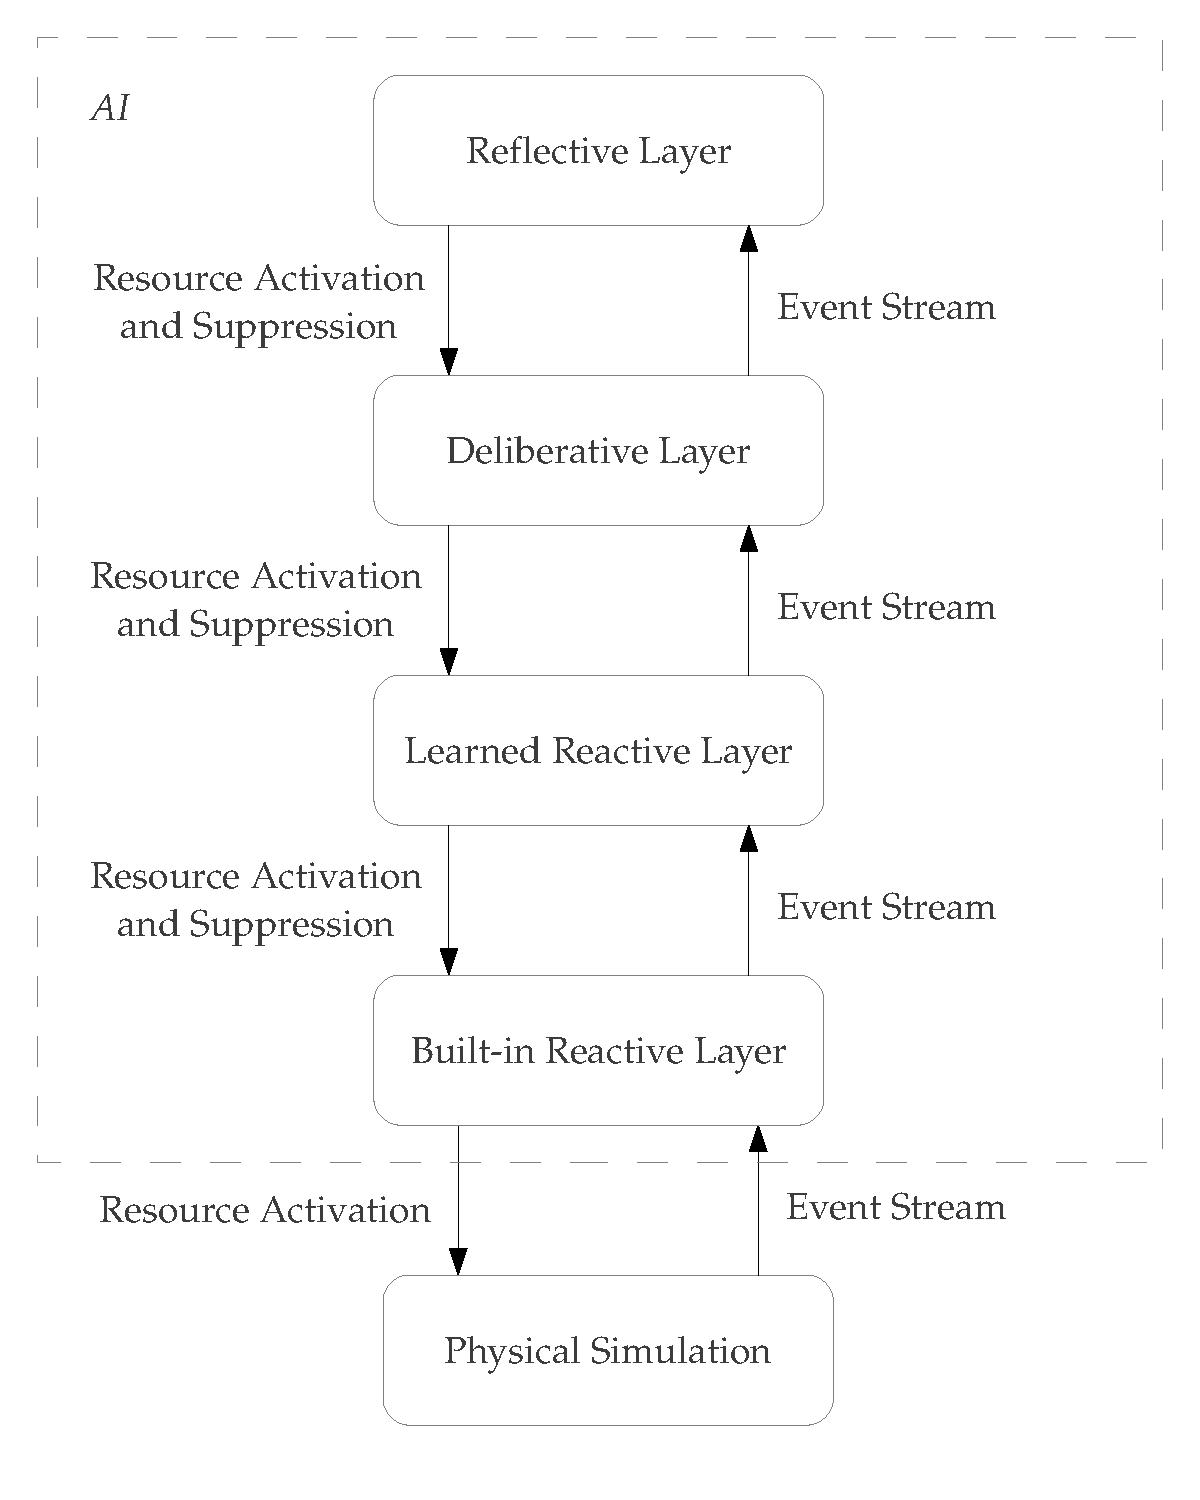
\includegraphics[width=10cm]{gfx/four_layers_overview}
\end{center}
\caption[The four layers of the AI in relation to the physical
  simulation.]{The layers of the AI in relation to the physical
  simulation.  The four layers of the AI form cascaded control loops,
  where each layer reflectively controls the layers below.}
\label{figure:four_layers_overview}
\end{figure}

In the following sections, I give an overview of the types of
knowledge and processes that comprise the physical simulation as well
as each of the four layers of reflective control in the AI that
simulate this example of reflectively learning not only to physically
act but also to deliberatively plan.  These following sections will
only be a cursory overview of the layers.  The AI is organized into
layers of reflection that are each themselves composed of
\emph{agencies} that are in turn composed of \emph{resources} that can
be controlled and executed concurrently by the layers above.

\section{The Physical Simulation}

The block building domain is implemented as a simulation based on
two-dimensional ridid-body physical laws, including floating point
numerical representations for object positions, velocities and
accelerations.  Changes in the semantic relationships between objects
in the physical simulation are sent in a stream of perceptual events
from the physical simulation to the AI.  The semantic relationships
that are computed by the physical simulation are basic visual
relationships, such as the prepositional relationships, ``$X$ is on
top of $Y$'' and ``$X$ is to the left of $Y$'', as well as visual
properties, such as ``$X$ is the color $Y$'' or ``$X$ has the shape
$Y$''.  This semantic visual knowledge is represented as frame-based
objects in the physical simulation, which reports any changes to this
knowledge to the AI as a stream of visual events.  For example, the
semantic knowledge can be thought of as a list of the following types
of subject-verb-object sentences:
\begin{itemize}
\item Block-1 is-a block.
\item Table-1 is-a table.
\item Gripper-1 is-a gripper.
\item Block-1 has-the-color blue.
\item Block-2 has-the-shape pyramid.
\item Block-1 is-on Table-1.
\item Block-2 is-on Table-1.
\item Gripper-1 is-holding Block-1.
\item Gripper-1 is-above Table-1.
\item Block-2 is-to-the-left-of Gripper-1.
\end{itemize}
The physical simulation generates a list of these simple
subject-verb-object sentences in its internal state.  The actual
internal lisp-like representation of the physical simulation is shown
in \autoref{table:internal_lisp_like_physical_representation}.
\begin{table}[h]
\begin{center}
{\fbox{
\begin{tabular}{l}
 {\tt{[Block-1 left-of Gripper-1]}} \\
 {\tt{[Block-1 on Table-1]}} \\
 {\tt{[Block-1 shape cube]}} \\
 {\tt{[Block-1 color blue]}} \\
 {\tt{[Block-1 is-a block]}} \\
 {\tt{[Block-2 right-of Gripper-1]}} \\
 {\tt{[Block-2 on Table-1]}} \\
 {\tt{[Block-2 shape pyramid]}} \\
 {\tt{[Block-2 color green]}} \\
 {\tt{[Block-2 is-a block]}} \\
 {\tt{[Table-1 left-of Gripper-1]}} \\
 {\tt{[Table-1 shape cube]}} \\
 {\tt{[Table-1 color white]}} \\
 {\tt{[Table-1 is-a table]}} \\
 {\tt{[Gripper-1 is-holding []]}} \\
 {\tt{[Gripper-1 color black]}} \\
 {\tt{[Gripper-1 is-a gripper]}} \\
 {\tt{[Gripper-1 movement\_command stop]}} \\
 {\tt{[Gripper-1 is me]}}
\end{tabular}
}}
\end{center}
\caption[Internal semantic visual representation generated by the body
  in the physical simulation.]{Internal semantic visual representation
  generated by the body in the physical simulation.  Changes to this
  representation are sent as a stream of visual change events to the
  built-in reactive layer of the AI.}
\label{table:internal_lisp_like_physical_representation}
\end{table}

\section{The Built-in Reactive Layer}

The physical simulation generates a stream of events that represent
changes in the perceptual state of the body of the AI.  The first
layer of the AI is \emph{the built-in reactive layer}, which monitors
this event stream of perceptual changes in object knowledge from the
physical simulation.  These changes in the perceptual state of the
AI's body in the physical simulation are reconstructed in the built-in
reactive layer.  In this way, the built-in reactive layer maintains a
representation of the visual knowledge that the body is currently
seeing.  The representation of the perceptual state of the body that
informs the AI about the physical world is referred to as \emph{the
  visual knowledge base}.  The built-in reactive layer also contains
predefined physical action resources that are available in the
physical body of the AI in the physical simulation.  Because the
built-in reactive layer is the primary interface to the physical body
that the AI controls, many of the resources of the built-in layer are
actually defined by the physical simulation during the initial boot-up
process of the entire AI-physical-simulation system.  Also, the
specific types of semantic visual objects and prepositional
relationships and properties are not known to the mind until they are
received from the physical simulation.  The AI simply expects to
receive a stream of visual objects, their relationships, and
properties.

\section{The Learned Reactive Layer}

Changes to the visual knowledge base in the built-in reactive layer
constitute the stream of events that \emph{the learned reactive layer}
receives and reconstructs into a more stable representation of the
physical world.  The AI's current representation of the physical world
is referred to as \emph{the physical knowledge base}.  I have found
the distinction between visual and physical knowledge to be useful in
domains where only partial information about the physical world is
available through the senses.  In this case, some reasoning must be
done in order to debug the physical knowledge when contradictory
visual input is detected.  For example, in a kitchen cooking domain
(see {\mbox{\autoref{figure:isis_world_two_agents}}}), the AI sees a
stick of butter in the refrigerator.  Subsequently, the AI sees the
same stick of butter on a table.  The AI must resolve the fact the
either (1) the table is small enough to fit into the refrigerator or
(2) the stick of butter is no longer in the refrigerator.  The
reactive layers of the AI that are necessary for navigating the
kitchen domain are factors that complicate explaining the deliberative
and reflective thinking layers of the AI.  The learning and planning
agencies of the deliberative and reflective thinking layers are
exactly the same for the block building domain as they are for the
kitchen domain.  Thus, I will focus on explaining the AI's reflective
thinking processes in terms of the simpler block building domain as
the reflective thinking capabilities are the focus of this thesis.  In
the block building domain, the physical knowledge base is a faithful
reconstruction of the visual knowledge base, slightly behind the
times.  {\mbox{\autoref{figure:implemented_physical_knowledge}}} shows
the physical knowledge base that is reconstructed from the reflective
change events that the learned reactive layer receives from changes in
the visual knowledge base of the built-in reactive layer.
\begin{figure}
\begin{center}
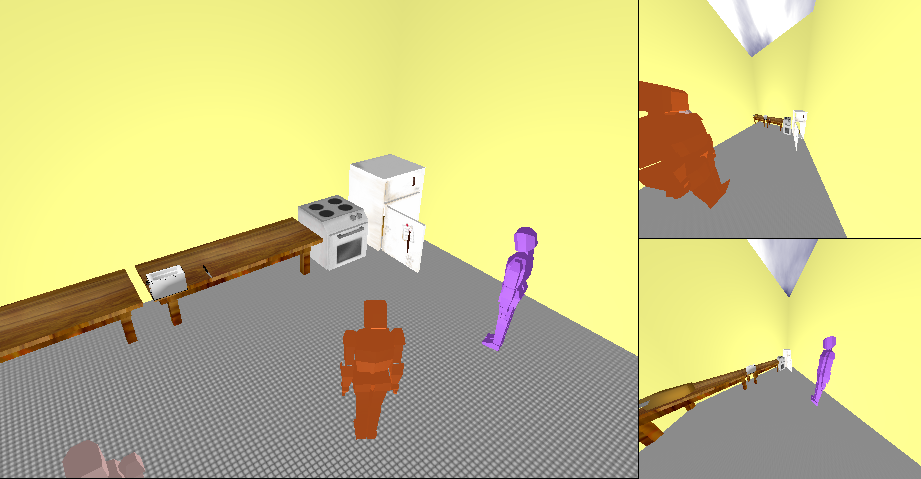
\includegraphics[width=12cm]{gfx/isis_world_two_agents}
\end{center}
\caption[Kitchen cooking domain with partial visual knowledge of the
  physical domain.]{Kitchen cooking domain with only partial visual
  knowledge of the physical domain available to the AI.  The image on
  the left is a bird's-eye-view of the situation, while the images on
  the right contain the objects that each AI can actually see.}
\label{figure:isis_world_two_agents}
\end{figure}
\begin{sidewaysfigure}
\begin{center}
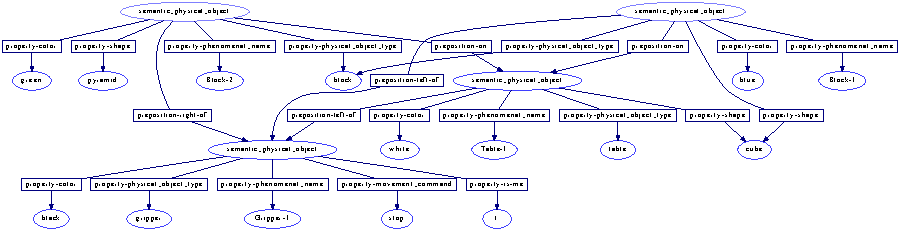
\includegraphics[width=8.5in]{gfx/implemented_physical_knowledge}
\end{center}
\hspace{4cm}\parbox{15cm}{\caption[The physical knowledge base.]{The
    physical
    knowledge base.}\label{figure:implemented_physical_knowledge}}
\end{sidewaysfigure}

\section{The Deliberative Layer}

\emph{The deliberative layer} receives a stream of events from the
learned reactive layer including changes to the physical knowledge
base as well as changes in the activation states of reactive
resources.  While the reactive layer may react to visual or physical
knowledge immediately, the deliberative layer learns models of this
reactive behavior at a more steady and often slower pace.  This allows
the reactive layer to operate at full speed, often in bursts of
activity, while a buffered stream of events is reasoned about more
carefully by the deliberative layer without slowing the primary
activity of physical reaction.  The deliberative layer first
reconstructs a copy of the physical knowledge base that it can use as
reference for the slower deliberative learning processes.  From this
reconstruction of the physical knowledge base, the deliberative layer
induces and counts common types of knowledge.  This type induction
process is focused only on the parts of the physical knowledge base
that have changed.  The deliberative layer stores counts of these
types of knowledge in a knowledge base in the deliberative layer
called \emph{the physical type knowledge base}.  The physical type
knowledge base counts the occurrences of types of knowledge in the
deliberative layer's reconstruction of the physical knowledge base.
{\mbox{\autoref{figure:physical_type_knowledge_induction}}} shows the
knowledge bases involved in the induction of physical type knowledge.
The following is a list of types of physical type knowledge that is
accounted for in the physical type knowledge base at any given point
in time:
\begin{itemize}
\item A block is sitting on another block.
\item A block with a pyramid shape is sitting on Block-1.
\item A green block is sitting on a blue block.
\item A block is to the left of a gripper.
\end{itemize}
\begin{figure}
\begin{center}
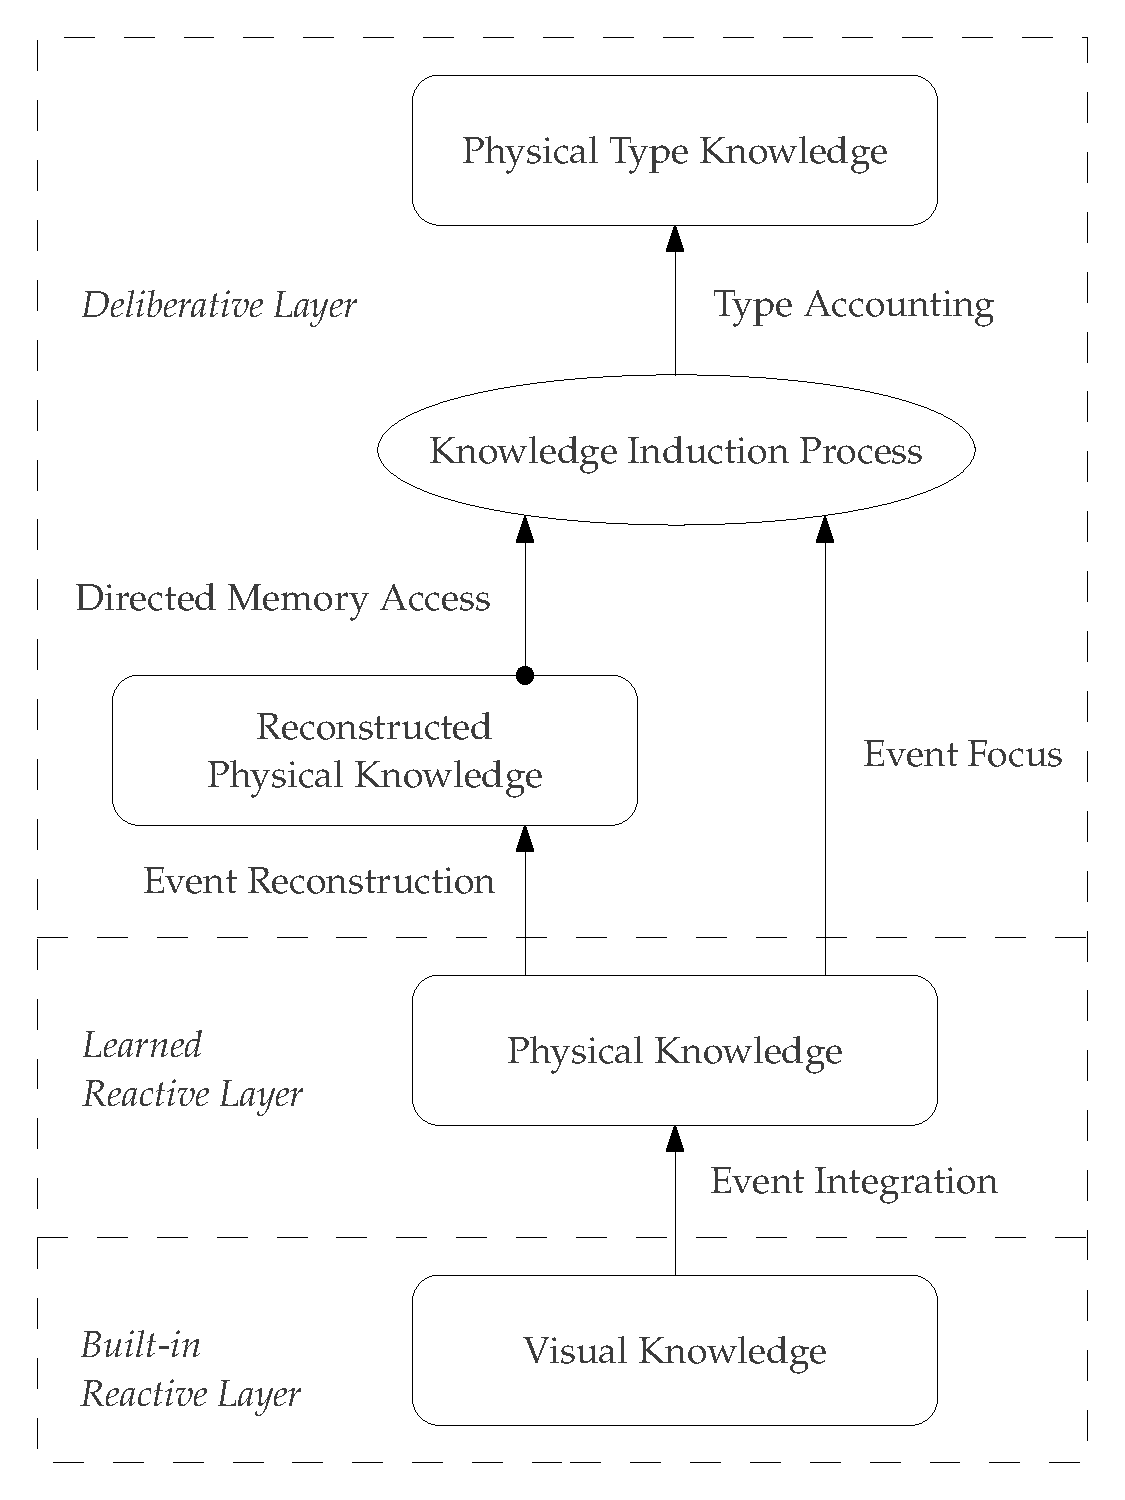
\includegraphics[width=10cm]{gfx/physical_type_knowledge_induction}
\end{center}
\caption[The knowledge bases involved in physical type knowledge
  induction.]{The knowledge bases involved in physical type knowledge
  induction.  The creation of a reconstruction of the physical
  knowledge base by the deliberative layer allows the full speed
  concurrent execution of the reactive layer, despite the slower speed
  of the more careful deliberative learning processes.}
\label{figure:physical_type_knowledge_induction}
\end{figure}

In addition to events about knowledge in the physical knowledge base
of the reactive layer, the deliberative layer also receives events
that specify the beginning and ending times of reactive layer resource
executions.  Resource execution events are causally traced, so that
execution call graphs are easily reconstructed asynchronously by the
deliberative layer.
{\mbox{\autoref{figure:implemented_reflective_event_knowledge_base}}}
shows a time-line visualization of the reflective event knowledge base
that is constructed from the execution events of the reactive
resources.  Once a beginning and an ending time for an execution event
in the reactive layer is received by the deliberative layer, a future
task is created to learn the physical type knowledge transframe for
this resource execution.  The learning of a physical type knowledge
transframe for the execution of a reactive resource must wait for the
physical type knowledge base to catch up with processing the current
information from the visual and physical knowledge bases in the
reactive layer.
\begin{figure}
\begin{center}
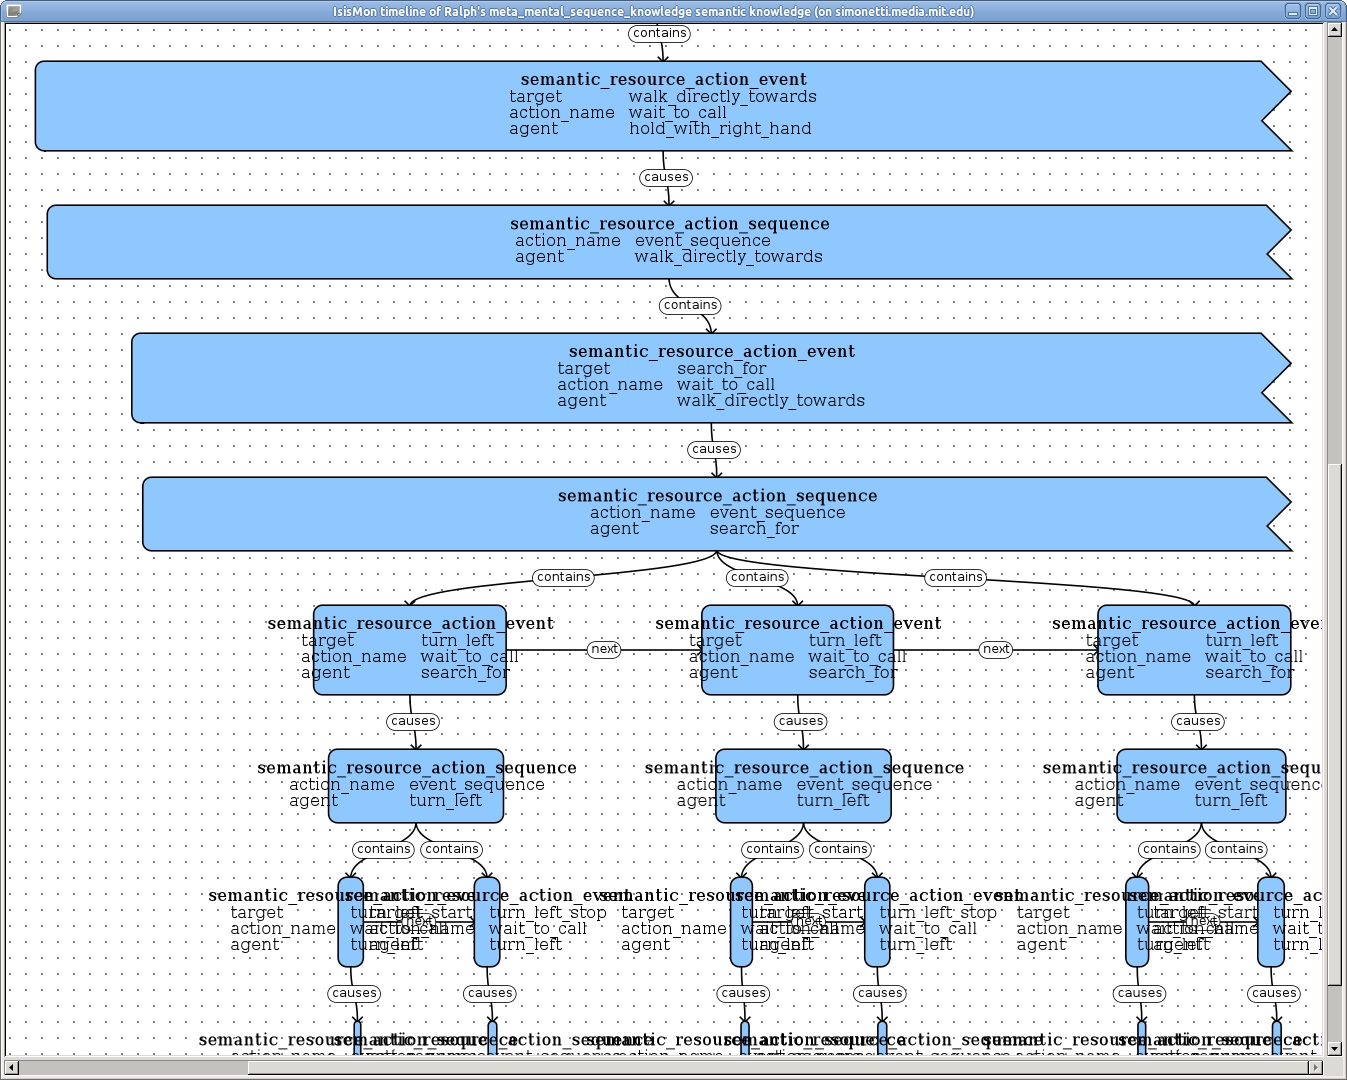
\includegraphics[width=10cm]{gfx/implemented_reflective_event_knowledge_base}
\end{center}
\caption[A time-line visualization of the reflective event knowledge
  base that is constructed from the execution events from the reactive
  resources.]{A time-line visualization of the reflective event
  knowledge base that is constructed from the execution events from
  the reactive resources has a hierarchical causal structure.  The
  horizontal axis represents time, while rounded rectangles represent
  execution events of different reactive resources.  Notice that some
  rectangles have a jagged right edge.  This represents that the event
  does not yet have an ending time.  Once an event has both a
  beginning and an ending time in this knowledge base, which a
  reflective process recognizes, the action transframe hypotheses are
  refined, given the new physical change correlations for the resource
  execution.}
\label{figure:implemented_reflective_event_knowledge_base}
\end{figure}

Once a physical type transframe is computed for a reactive event, a
version space concept learning algorithm \cite[]{mitchell:1997} is
created for each add or remove physical type knowledge change in the
transframe.  In the concept learning algorithm, a conjunctive
hypothesis space of predictive physical type preconditions is
represented in terms of a version space generalization lattice, so
that all possibly correct hypotheses that predict the transframe
change evidence are represented in a relatively compact way.  Once a
hypothesis space is created for a transframe change, this hypothesis
space is associated with the reactive action so that it may be used by
the deliberative layer to infer the counterfactual results of
executing the action in its planning machine.
{\mbox{\autoref{table:abstract_physical_transframe}}} shows an example
of a physical type knowledge transframe based on the changes in the
physical type knowledge base over time.
\begin{table}[h]
\centering
\begin{tabular}{c}
  Hypothesized Physical Type Knowledge Transframe for Action \\
  \begin{tabular}{|l|l|}
    \hline
    \emph{action:}        & Reach and grab. \\
    \hline
    \emph{preconditions:} & A block is below a gripper. \\
    ~                     & A gripper is holding nothing. \\
    \hline
    \emph{additions:}     & A gripper is holding a block. \\
    \hline
    \emph{removals:}      & A gripper is holding nothing. \\
    \hline
  \end{tabular}
\end{tabular}
\caption[Hypothesized physical type knowledge transframe for
  action.]{Hypothesized physical type knowledge transframe including
  action dependent sets of physical type knowledge \emph{add} and
  \emph{remove} changes with learned conjunctive hypothesis spaces
  based on a set of physical type knowledge preconditions.}
\label{table:abstract_physical_transframe}
\end{table}

In order to learn transframes from physical type knowledge, it is
useful to have the physical type knowledge base able to be indexed at
arbitrary points in the past.  This is achieved by representing
physical type knowledge in the form of events that have beginning and
ending times.  All events in the physical type knowledge base are
automatically organized into an interval tree, so that any temporal
indexing of the physical type knowledge base can be done with $O(\log
n)$ time complexity as $n$ increases linearly with the number of
physical type knowledge events in the knowledge base.  Thus, computing
the physical type knowledge transframe between any two points in the
past can be done relatively quickly.  A necessary feature that must
still be added to the architecture is a \emph{forgetful} physical type
knowledge base.  There are many forgetful event streams in the
language, and the ability to treat an entire event knowledge base as a
forgetful streaming object is a way to allow this knowledge base to
not grown indefinitely over the run-time of the algorithm.

Once the deliberative layer learns action dependent transframe
hypotheses in terms of the physical type knowledge, these hypotheses
can be used for imagining the hypothetical types of effects of
actions.  This hypothetically supported knowledge is stored by the
deliberative layer in \emph{the counterfactual physical type knowledge
  base}.  The counterfactual physical type knowledge is used for
imagining the execution of plans, a step in the planning process.
Plans sometimes assert conditions in the physical type knowledge base.
During the imagination of the plan execution, the counterfactual
physical type knowledge is used for determining whether assertions
will succeed or fail in the imagination of the plan's counterfactual
execution knowledge.  For example,
{\mbox{\autoref{table:a_plan_learned_from_being_told}}} on
{\mbox{page~\pageref{table:a_plan_learned_from_being_told}}} shows a
plan that contains the assertion that ``a cube is sitting on a
pyramid''.  The AI has no experience executing this plan because it
has only ``been told'' this plan.  The AI adds the types of knowledge
asserted within the plan to the possible hypothetical transframes for
the actions in the plan.  This causes the AI to have a concept learner
for predicting the change that would satisfy the assertion in the
plan.  Inferred counterfactual physical type knowledge can predict
both that an action in the plan will cause the knowledge necessary for
the assertion to succeed as well as that the knowledge for the
assertion will not be caused and the assertion will fail.  Notice that
even if a plan fails given certain preconditions, there is always the
potential that this plan will successfully complete under some
possible future preconditions.  The utility of the plan is learned
through experiences in different physical type preconditions.  In this
way, the inferred hypothetical effects of an action can be learned
from ``being told'' as well as eliminated through experience executing
the plan.

Finally, the deliberative layer goes through a list of the plans that
it knows and imagines executing them.  If the imagined plan succeeds
and accomplishes the physical type goals of the deliberative planning
machine, then the plan is executed.  The deliberative planning machine
has the following goal: ``A block is sitting on a block.''  When the
AI imagines executing the plan in
{\mbox{\autoref{table:a_plan_learned_from_being_told}}} on
{\mbox{page~\pageref{table:a_plan_learned_from_being_told}}}, there is
hypothetical support for the counterfactual knowledge: ``A cube is
sitting on a pyramid.''  The deliberative imagination agency infers
the hypothetical effects of the plan.  The counterfactual physical
type knowledge base contains the assertion of the plan, an instance of
the current physical type goal, ``A block is sitting on a block.''
Since the goal is hypothetically supported, the plan is executed by
the deliberative execution agency.  The experienced gained from
actually executing the plan results in the learning of a more refined
model of the physical world as well as a more refined model of the
deliberative planning machine.  The details of how the deliberative
infers hypothetically supported counterfactual knowledge so that it
can be corrected as hypotheses are refined in the learning process is
described in detail in the next chapter,
\autoref{chapter:grounded_learning_of_knowledge_utility},
``\nameref{chapter:grounded_learning_of_knowledge_utility}.''

\section{The Reflective Layer}

While the deliberative layer learns hypothetical models of how
physical actions affect the types of physical knowledge, the
reflective layer learns hypothetical models of how deliberative
actions affect the types of deliberative knowledge.  The reflective
layer receives a stream of deliberative planning machine knowledge
events, which it uses to reconstruct a copy of the deliberative
planning machine knowledge base that it can use for inducing
deliberative type knowledge at a steadier pace than the shorter-lived
``bursty'' executions of the deliberative planning machine resources.
The deliberative planning machine knowledge base does not contain
physical objects but instead contains deliberative objects, such as
the planning machine, goals, plans, and failure events.
{\mbox{\autoref{figure:deliberative_planning_machine_knowledge_base}}}
shows the deliberative planning machine knowledge base that the
reflective layer concurrently reconstructs from a procedural events
stream and learns hypotheses for how to control by imagining plans
involving the deliberative planning resources.
\begin{sidewaysfigure}
  \begin{tabular}{p{8in}}
    % define source coordinates
    \begin{itemize}
    \item Plan for Physical Action in Deliberative Planning Machine Focus Register \tikz[na] \coordinate (executing-plan-label);
    \item Plan for Physical Action in Deliberative Planning Machine Execute Register \tikz[na] \coordinate (focus-plan-label);
    \item Deliberative Planning Machine \tikz[na] \coordinate (deliberative-planning-machine-label);
    \end{itemize} \\
    % Use a background grid to make it easier to find coordinates
    % When the coordinates have been found, remove the 
    % 'show background grid' option. 
    %\tikzstyle{background grid}=[draw, black!50,step=.5cm]
    \begin{tikzpicture}%[show background grid]
      % Put the graphic inside a node. This makes it easy to place the
      % graphic and to draw on top of it. 
      % The above right option is used to place the lower left corner
      % of the image at the (0,0) coordinate. 
      
      \node [inner sep=0pt,above right] {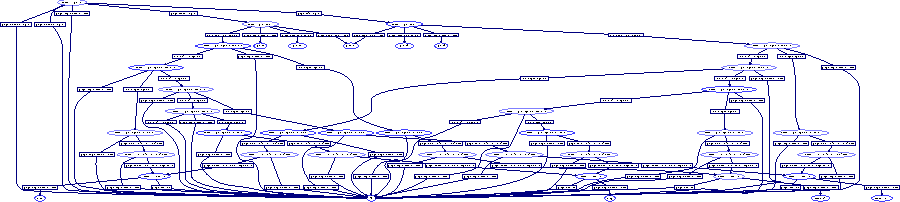
\includegraphics[width=8in]{gfx/deliberative_planning_machine_knowledge_base}};
      
      % show origin
      %\fill (0,0) circle (2pt);
      % define destination coordinates
      \path (17.5,2) coordinate (executing-plan)
      (6,2.25) coordinate (focus-plan)
      (1.75,4.5) coordinate (deliberative-planning-machine);
    \end{tikzpicture}
  \end{tabular}
  
  % define overlays
  % Note the use of the overlay option. This is required when 
  % you want to access nodes in different pictures.
  \begin{tikzpicture}[overlay]
    \draw (executing-plan) node[ellipse, dashed, dash pattern=on 10pt off 10pt, red, minimum height=4cm,minimum width=6cm, line width=1.5, draw] {};
    \path[->,red,thick, line width=1.5] (executing-plan-label) edge [out=0, in=120] (executing-plan);
    
    \draw (focus-plan) node[ellipse, dashed, dash pattern=on 10pt off 10pt, red, minimum height=4cm,minimum width=6cm, line width=1.5, draw] {};
    \path[->,red,thick, line width=1.5] (focus-plan-label) edge [out=0, in=60] (focus-plan);
    
    \draw (deliberative-planning-machine) node[ellipse, dashed, dash pattern=on 10pt off 10pt, red, minimum height=0.5cm,minimum width=1.5cm, line width=1.5, draw] {};
    \path[->,red,thick, line width=1.5] (deliberative-planning-machine-label) edge [out=0, in=-60] (deliberative-planning-machine);
  \end{tikzpicture}
  \hspace{4cm}\parbox{15cm}{\caption[The deliberative planning machine
      knowledge base with the deliberative planning machine and two
      plans.]{The deliberative planning machine knowledge base with
      the deliberative planning machine and two plans are circled.
      These plans are each on one of the planning machine's registers,
      the \emph{focus} register and the \emph{execution}
      register.}\label{figure:deliberative_planning_machine_knowledge_base}}
\end{sidewaysfigure}

The reflective layer learns to make plans for accomplishing and
avoiding types of deliberative knowledge states.  Analagously to how
physical type knowledge is induced from the specific physical states,
the reflective layer induces types of deliberative planning machine
knowledge from the specific deliberative planning machine states.  If
a specific planning machine state is ``Plan-1 is in
Planning-Machine-1's focus register and has had the failure
Expectation-Failure-1,'' the following type knowledge can be induced
from this specific state: ``A plan is in a planning machine's focus
register,'' and ``A plan has had a failure.''
{\mbox{\autoref{figure:deliberative_type_knowledge_induction}}} shows
an overview of the knowledge bases and processes involved in the
induction of the deliberative planning machine type knowledge base
from the deliberative planning machine knowledge base by the
reflective layer.  The reflective layer uses an analogous type
knowledge induction process as the deliberative layer, previously
shown in {\mbox{\autoref{figure:physical_type_knowledge_induction}}}
on {\mbox{page~\pageref{figure:physical_type_knowledge_induction}}}.
\begin{figure}[h]
\centering
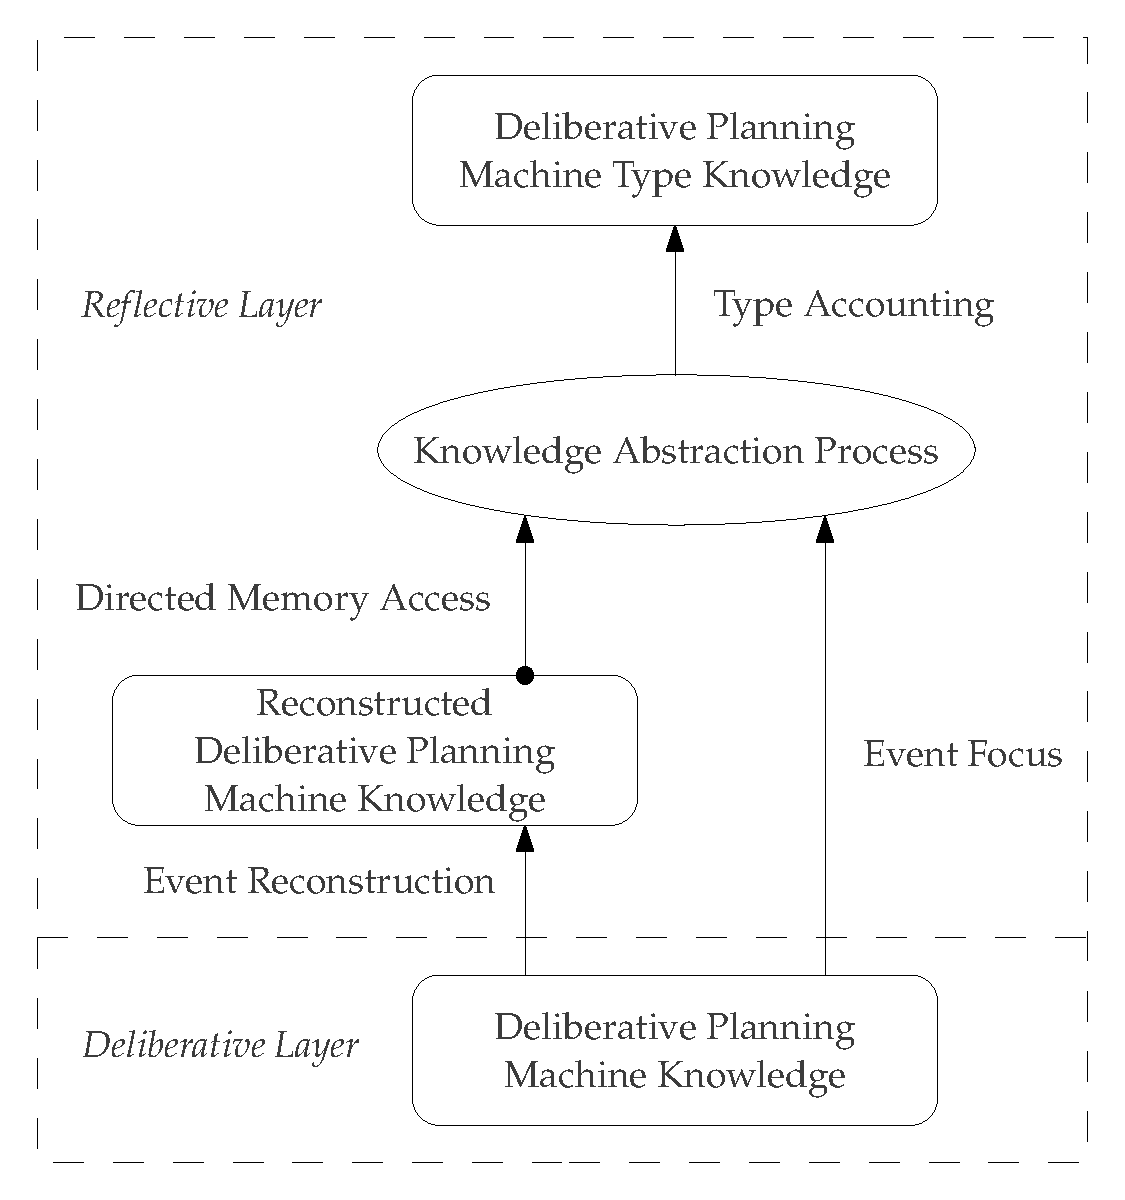
\includegraphics[width=10cm]{gfx/deliberative_type_knowledge_induction}
\caption[The knowledge bases and processes involved in deliberative
  planning machine type knowledge induction.]{The knowledge bases and
  processes involved in deliberative planning machine type knowledge
  induction.  The creation of a reconstruction of the deliberative
  planning machine knowledge base by the reflective layer allows the
  full speed concurrent execution of the deliberative planning
  machine, despite the slower speed of the more careful reflective
  learning processes.}
\label{figure:deliberative_type_knowledge_induction}
\end{figure}

Plans in the reflective planning machine knowledge base are imagined
in terms of the deliberative type knowledge.  This allows the
reflective layer planning machine to learn models of plan execution
that have no physical simulation component.  The ability to imagine
executing a plan and predicting its failure based on the structure of
the plan in relation to the planning machine and not in terms of the
physical world, is \emph{not} an advantage provided by physical
knowledge induction.  In this case, the ability to reason abstractly
about physical plans for action without any physical simulation
component necessary is provided by the reflective planning machine in
the reflective layer.  Hypotheses are learned by the reflective layer
that predict plan failure due to conjunctions of deliberative type
knowledge features.  One of the hypothetical deliberative type
knowledge transframes that the AI learns is the example expectation
failure is shown in
{\mbox{\autoref{table:hypothesized_deliberative_transframe}}}.
\begin{table}[h]
\centering
\begin{tabular}{c}
  Hypothesized Deliberative Type Knowledge Transframe for Action \\
  \begin{tabular}{|l|p{8cm}|}
    \hline
    \emph{action:}        & Execute and wait to complete. \\
    \hline
    \emph{preconditions:} & A plan is in focus that asserts a cube is sitting on a pyramid. \\
    ~                     & No plans have failed. \\
    \hline
    \emph{additions:}     & A plan has that just encountered a failure encountered an expectation failure. \\
    \hline
    \emph{removals:}      & No plans have failed. \\
    \hline
  \end{tabular}
\end{tabular}
\caption[Hypothesized deliberative type knowledge transframe for
  action.]{Hypothesized deliberative type knowledge transframe
  including action dependent sets of deliberative type knowledge
  \emph{add} and \emph{remove} changes with learned conjunctive
  hypothesis spaces based on a set of deliberative type knowledge
  preconditions.}
\label{table:hypothesized_deliberative_transframe}
\end{table}

The details of how the deliberative and reflective layers infer
hypothetically supported counterfactual knowledge so that it can be
corrected as hypotheses are refined in the learning process is
described in terms of detailed examples in the next chapter,
\autoref{chapter:grounded_learning_of_knowledge_utility},
``\nameref{chapter:grounded_learning_of_knowledge_utility}.''




